\section{Piecewise Quadratic Model with Hyperparameters}

Now we will attempt to imitate the effects of the parameter $E_0$ on the branches $f_\B$ and $f_\D$ better.
Previously, we just varied $c_R$ which changes the values of the whole branches evenly.
Now, we only want to affect the value at the left borders of these branches.
For this, we introduce new parameters that are tied directly to characteristics of the model function.

\subsection{Parameter Definitions}

The new parameters are $g_R\left(\frac{1}{4}\right)$ for the value at the left border of branches $f_\B$ and $f_\D$, $g_R\left(\frac{1}{2}\right)$ for the value at the right border of the branches, and finally $\left. \frac{d}{dx} g_R(x) \right|_{x = \frac{1}{2}}$ for the slope of the branches at the right border.
We fix the parameter $\left. \frac{d}{dx} g_R(x) \right|_{x = \frac{1}{2}} = 1.2$.
This way, the steepest slope is 1.2 which is just above 1.
Therefore, most of the function is still contractive.
We also fix the parameter $g_R\left(\frac{1}{2}\right) = \frac{1}{2} + \epsilon$ with $\epsilon = 0.025$ to have the value at the right border of the branches just above the bisector $y = x$.
The parameter left is $g_R\left(\frac{1}{4}\right)$, the value at the left border of the branches.
This parameter is varied.

\begin{subequations}
	\begin{align}
		g_R\left(\frac{1}{4}\right)                                     & = a_R \cdot \left(\frac{1}{4}\right)^2 + b_R \cdot \left(\frac{1}{4}\right) + c_R = \dfrac{a_R}{16} + \dfrac{b_R}{4} + c_R \label{equ:setup.quad.hyper.A} \\
		g_R\left(\frac{1}{2}\right)                                     & = a_R \cdot \left(\frac{1}{2}\right)^2 + b_R \cdot \left(\frac{1}{2}\right) + c_R = \dfrac{a_R}{4} + \dfrac{b_R}{2} + c_R \label{equ:setup.quad.hyper.B}  \\
		\left. \frac{d}{dx} g_R\left(x\right) \right|_{x = \frac{1}{2}} & = 2 \cdot a_R \cdot \left(\frac{1}{2}\right) + b_R \label{equ:setup.quad.hyper.C}
	\end{align}
\end{subequations}

\Crefrange{equ:setup.quad.hyper.A}{equ:setup.quad.hyper.A} are the values of $g_R\left(\frac{1}{4}\right), g_R\left(\frac{1}{2}\right),$ and $\left. \frac{d}{dx} g_R\left(x\right) \right|_{x = \frac{1}{2}}$.
This is a system of equations, we now need to solve for the parameters $a_R, b_R,$ and $c_R$.
To compute the parameters, we write the system as a matrix and invert it.
The matrix and its inverse are in \Cref{equ:setup.quad.hyper.matrix}.

\begin{align}
	\begin{pmatrix}
		\frac{1}{16} & \frac{1}{4} & 1 \\
		\frac{1}{4}  & \frac{1}{2} & 1 \\
		1            & 1           & 0
	\end{pmatrix}^{-1} & =
	\begin{pmatrix}
		16  & -16 & 4           \\
		-16 & 16  & -3          \\
		4   & -3  & \frac{1}{2}
	\end{pmatrix}
	\label{equ:setup.quad.hyper.matrix}
\end{align}

Hence, the equations for $a_R, b_R,$ and $c_R$ in dependence of $g_R\left(\frac{1}{4}\right), g_R\left(\frac{1}{2}\right),$ and $\left. \frac{d}{dx} g_R\left(x\right) \right|_{x = \frac{1}{2}}$ are \Crefrange{equ:setup.quad.hyper.aR}{equ:setup.quad.hyper.cR}.

\begin{align}
	a_R & = 16 \cdot g_R\left(\frac{1}{4}\right) - 16 \cdot g_R\left(\frac{1}{2}\right) + 4 \cdot \left. \frac{d}{dx} g_R\left(x\right) \right|_{x = \frac{1}{2}}     \label{equ:setup.quad.hyper.aR}     \\
	b_R & = -16 \cdot g_R\left(\frac{1}{4}\right) + 16 \cdot g_R\left(\frac{1}{2}\right) - 3 \cdot \left. \frac{d}{dx} g_R\left(x\right) \right|_{x = \frac{1}{2}} \label{equ:setup.quad.hyper.bR}        \\
	c_R & = 4 \cdot g_R\left(\frac{1}{4}\right) - 3 \cdot g_R\left(\frac{1}{2}\right) + \frac{1}{2} \cdot \left. \frac{d}{dx} g_R\left(x\right) \right|_{x = \frac{1}{2}} \label{equ:setup.quad.hyper.cR}
\end{align}

\subsection{Steep Parabola-shaped Branches $f_\A$ and $f_\C$}
\label{sec:setup.quad.hyper.1}

The values of the \hl{composite} parameters $g_R\left(\frac{1}{4}\right)$ and $\left. \frac{d}{dx} g_R\left(x\right) \right|_{x = \frac{1}{2}}$ are fixed as described previously in \Cref{sec:setup.quad.hyper.params}.
In this section, the values of the parameters of the function $g_L$ are set to $a_L = 8$ and $b_L = -1$ to get steep, shifted parabola-shaped branches $f_\A$ and $f_\D$, as one can see in the cobweb diagrams in \Cref{fig:setup.quad.hyper.1.cobwebs}.
Scanning the periods for reasonable values of $\alpha = g_R\left(\frac{1}{4}\right)$ and the parameter $\beta = c_L$ results in \Cref{fig:setup.quad.hyper.1.period}.
The reasonable values for $\alpha = g_R\left(\frac{1}{4}\right)$ are larger than $\frac{1}{4}$ to keep the parabola above the bisector $y = x$ and smaller than $\frac{1}{2}$ to keep the value of the model function at the left borders of the branches $f_\B$ and $f_\D$ below the value of the model function at the right borders.
For the specified values of $a_L$ and $b_L$, the reasonable values for $\beta = c_L$ are smaller than $0.22$ to not map the points directly onto the branch $f_\C$ from the branch $f_\A$.
To keep the parabola above the bisector $y = x$, the values for $\beta$ should also be larger than $0.12$.

With the newly chosen fixed parameters and the new \hl{composite} parameters, this model imitates the shape of the original model function well still.
The parameter $c_L$ is also still varied and this emulates the effects of $\chi_0$ on the branches $F_\A$ and $F_\C$ of the original model function well, as described in the previous section, \Cref{sec:setup.quad}.
The other varied parameter is the \hl{composite} parameter $g_R\left(\frac{1}{4}\right)$.
For brevity the varied parameters are named $\alpha = g_R\left(\frac{1}{4}\right)$ and $\beta = c_L$.
Varying the parameter $\alpha$ is a major improvement for emulating the effects of $E_0$ on the branches $F_\B$ and $F_\D$ of the original model function.
Increasing $\alpha$ primarily increases the values of the model function on the left sides of the branches $f_\B$ and $f_\D$ and keeps the values on the right sides the same.
It also moves the local minima of those branches to the left and decreases the value of the model function at those points, just as the parameter $E_0$ did to the original model function.

\begin{figure}
	\centering
	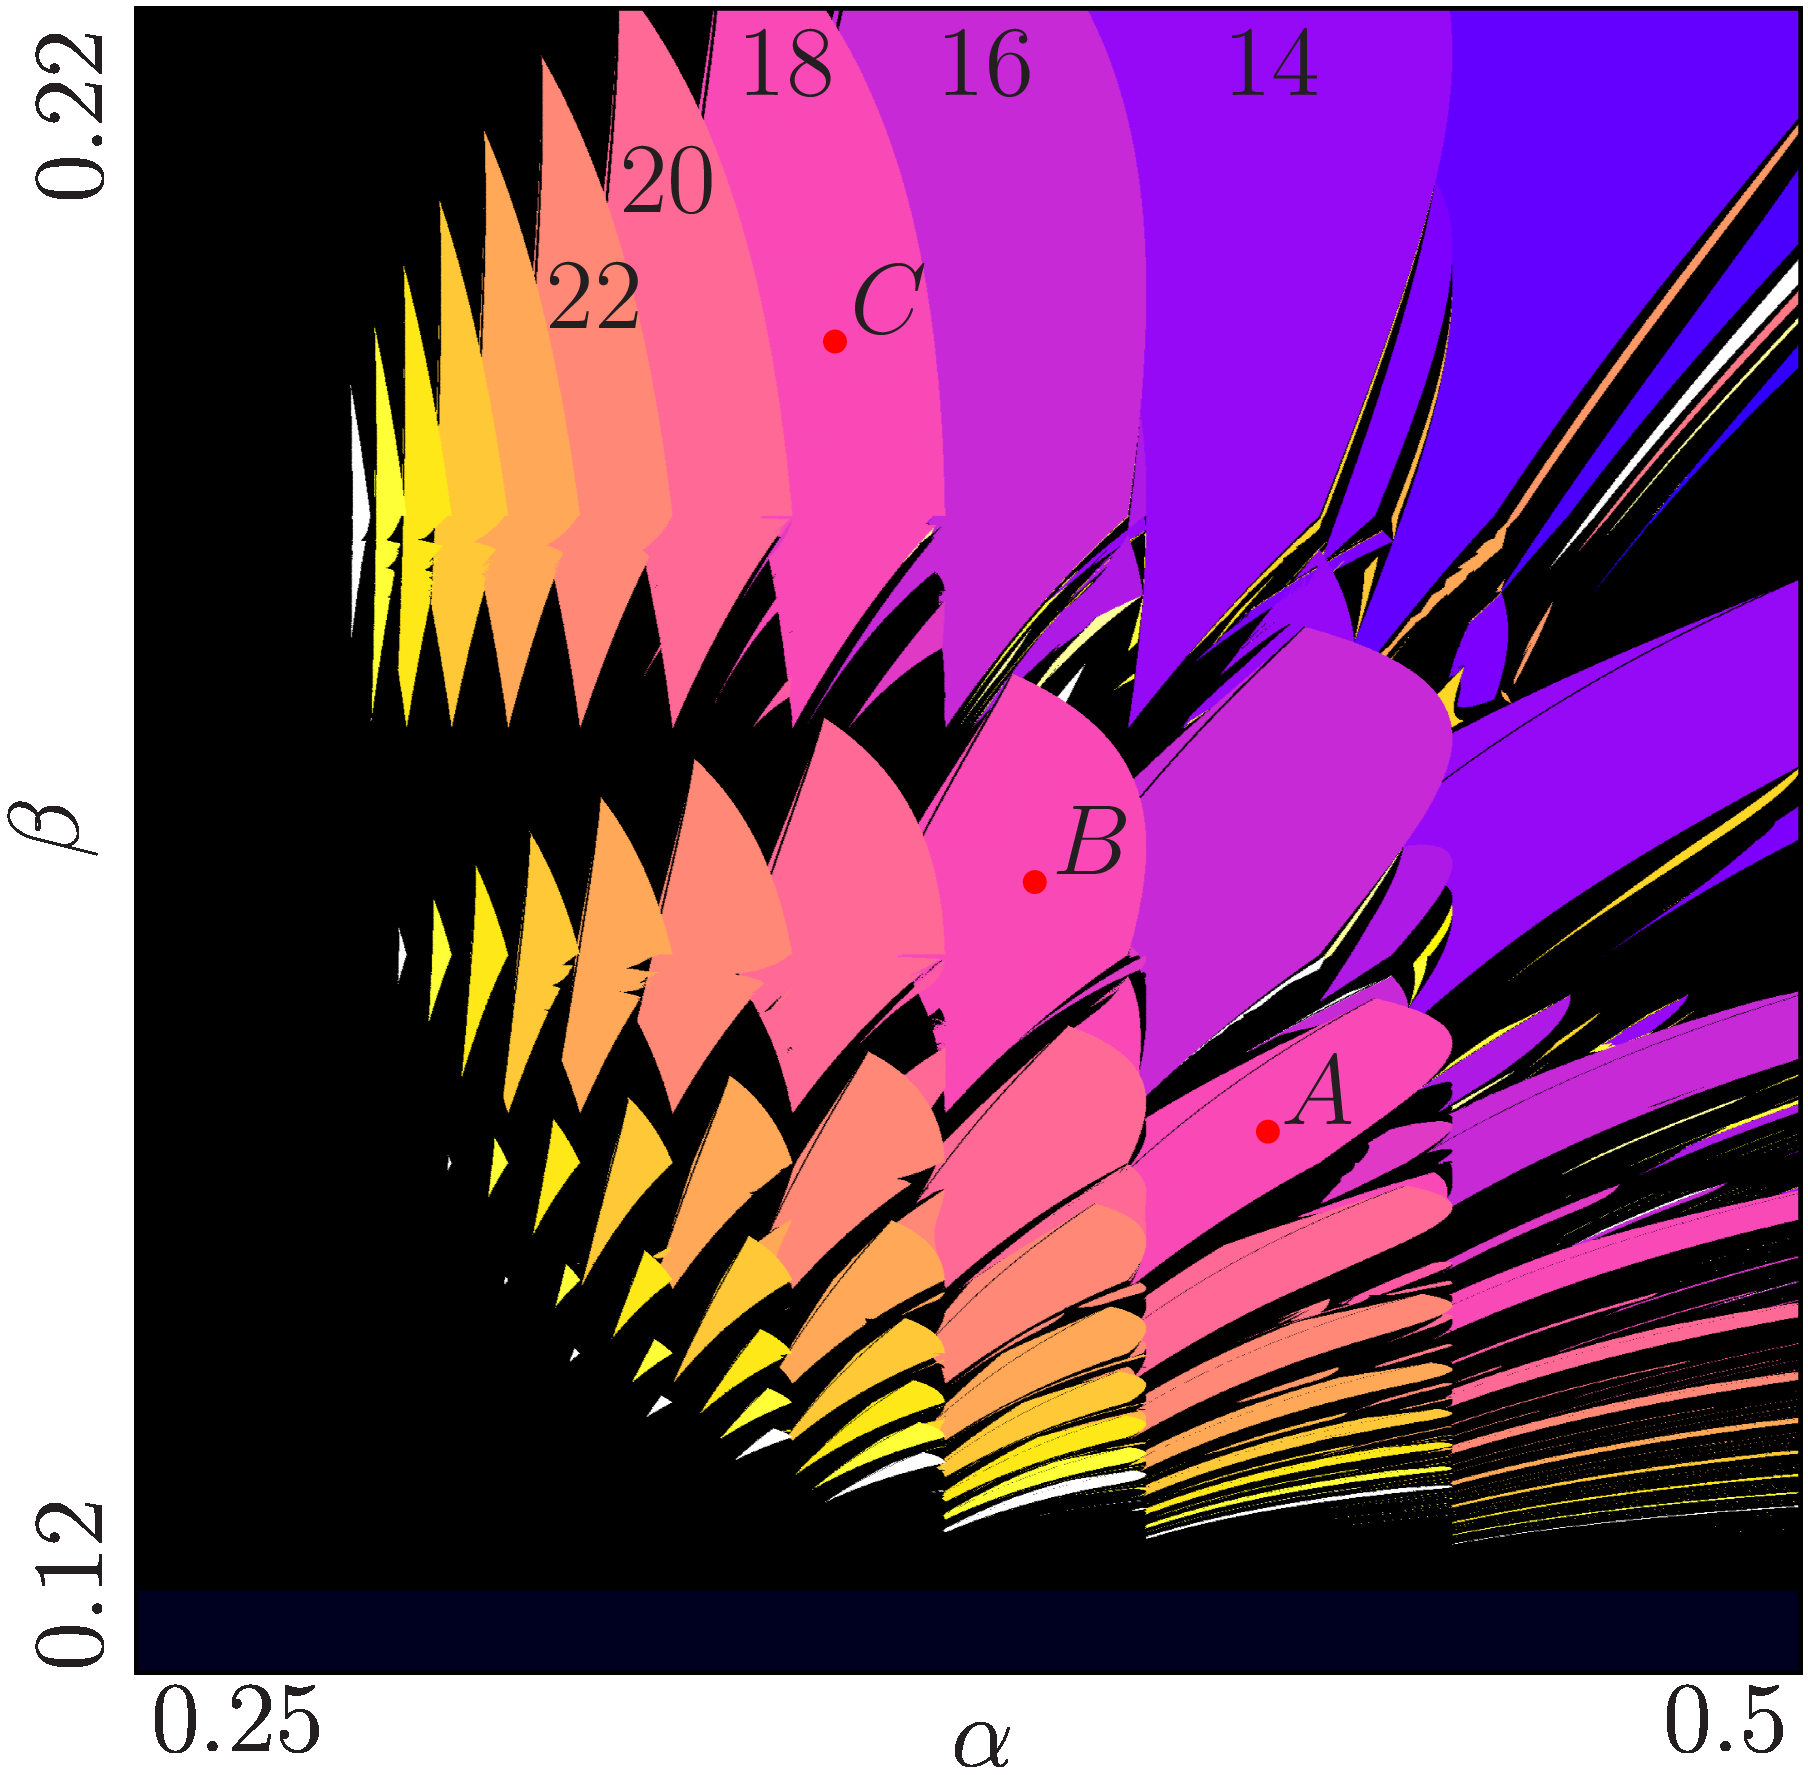
\includegraphics[width=0.6\textwidth]{../Figures/5/5.9/result.png}
	\caption[2D scan of the periods of the quadratic model with composite parameters]{
	2D scan of the periods of the piecewise quadratic model with \hl{composite} parameters $g_R\left(\frac{1}{4}\right), g_R\left(\frac{1}{2}\right),$ and $\left. \frac{d}{dx} g_R\left(x\right) \right|_{x = \frac{1}{2}}$.
	The parameters $a_L = 8, b_L = -1, g_R\left(\frac{1}{2}\right) = \frac{1}{2} + \frac{1}{40},$ and $\left. \frac{d}{dx} g_R\left(x\right) \right|_{x = \frac{1}{2}} = 1.2$ are fixed.
	The parameters $\alpha = g_R\left(\frac{1}{4}\right)$ and $\beta = c_L$ are varied in the ranges $[0.25, 0.5]$ and $[0.12, 0.22]$, respectively.
	The points $A, B,$ and $C$ mark the parameter values used for the cobweb diagrams in \Cref{fig:setup.quad.hyper.1.cobwebs}.
	Also, the numbers at the top indicate the period associated with some parameter regions.
	}
	\label{fig:setup.quad.hyper.1.period}
\end{figure}

\begin{figure}
	\centering
	\subfloat[$A$]{
		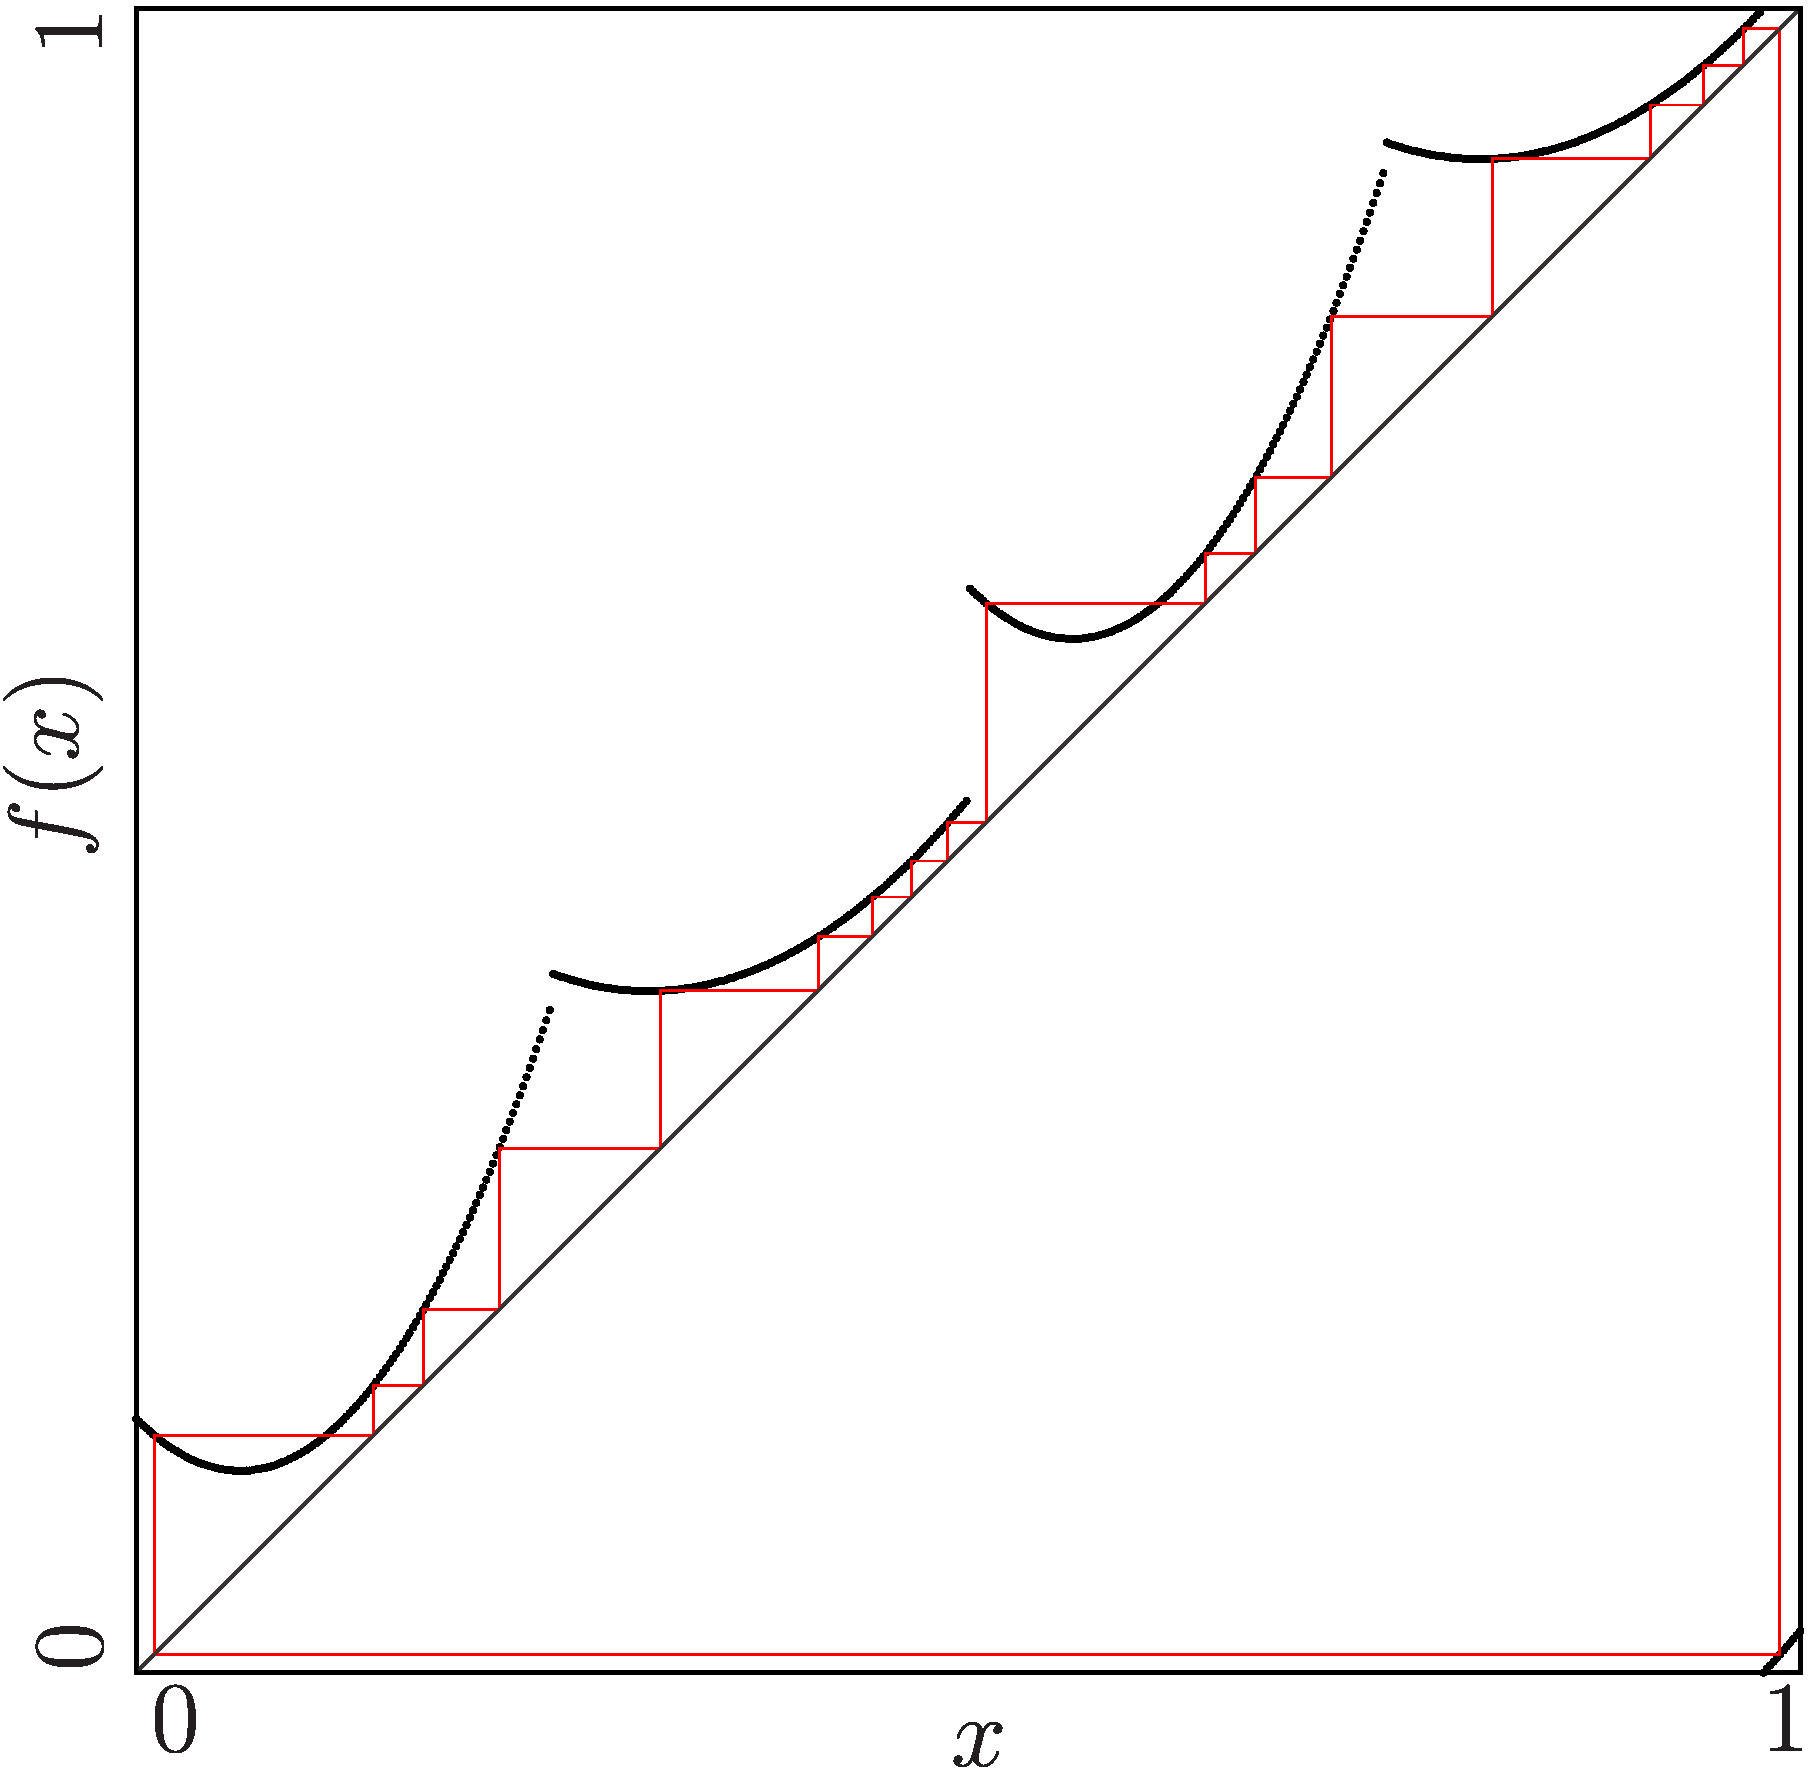
\includegraphics[width=.3 \textwidth]{../Figures/5/5.10a/result.png}
		\label{fig:setup.quad.hyper.1.cobweb.A}
	}
	\subfloat[$B$]{
		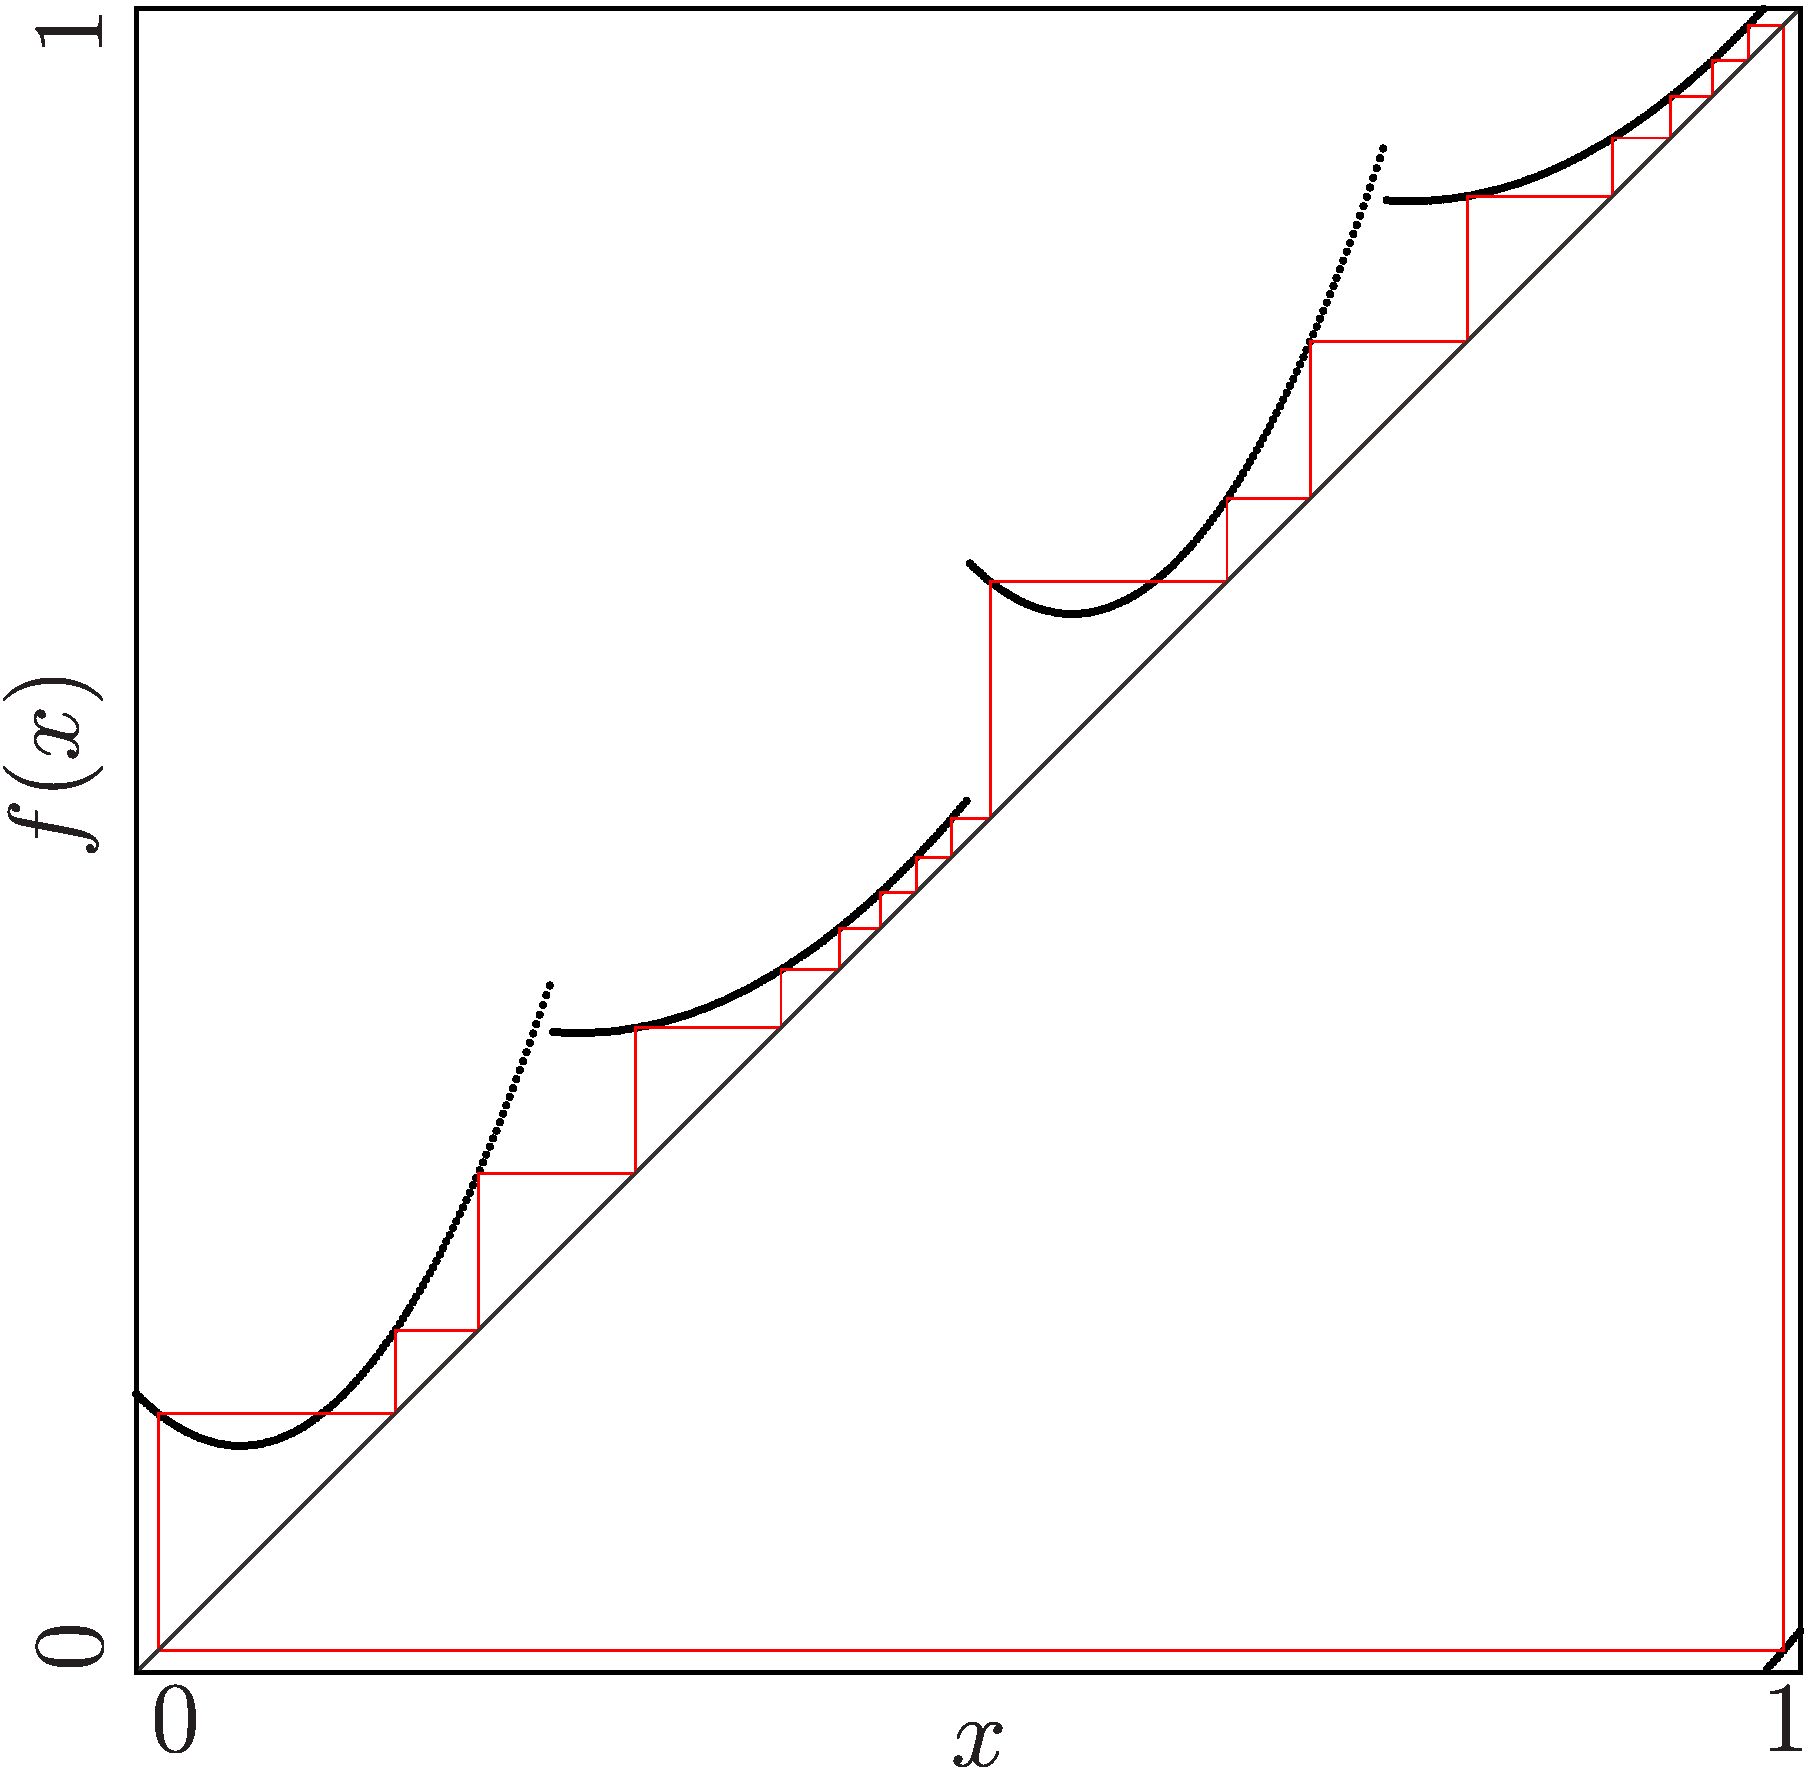
\includegraphics[width=.3 \textwidth]{../Figures/5/5.10b/result.png}
		\label{fig:setup.quad.hyper.1.cobweb.B}
	}
	\subfloat[$C$]{
		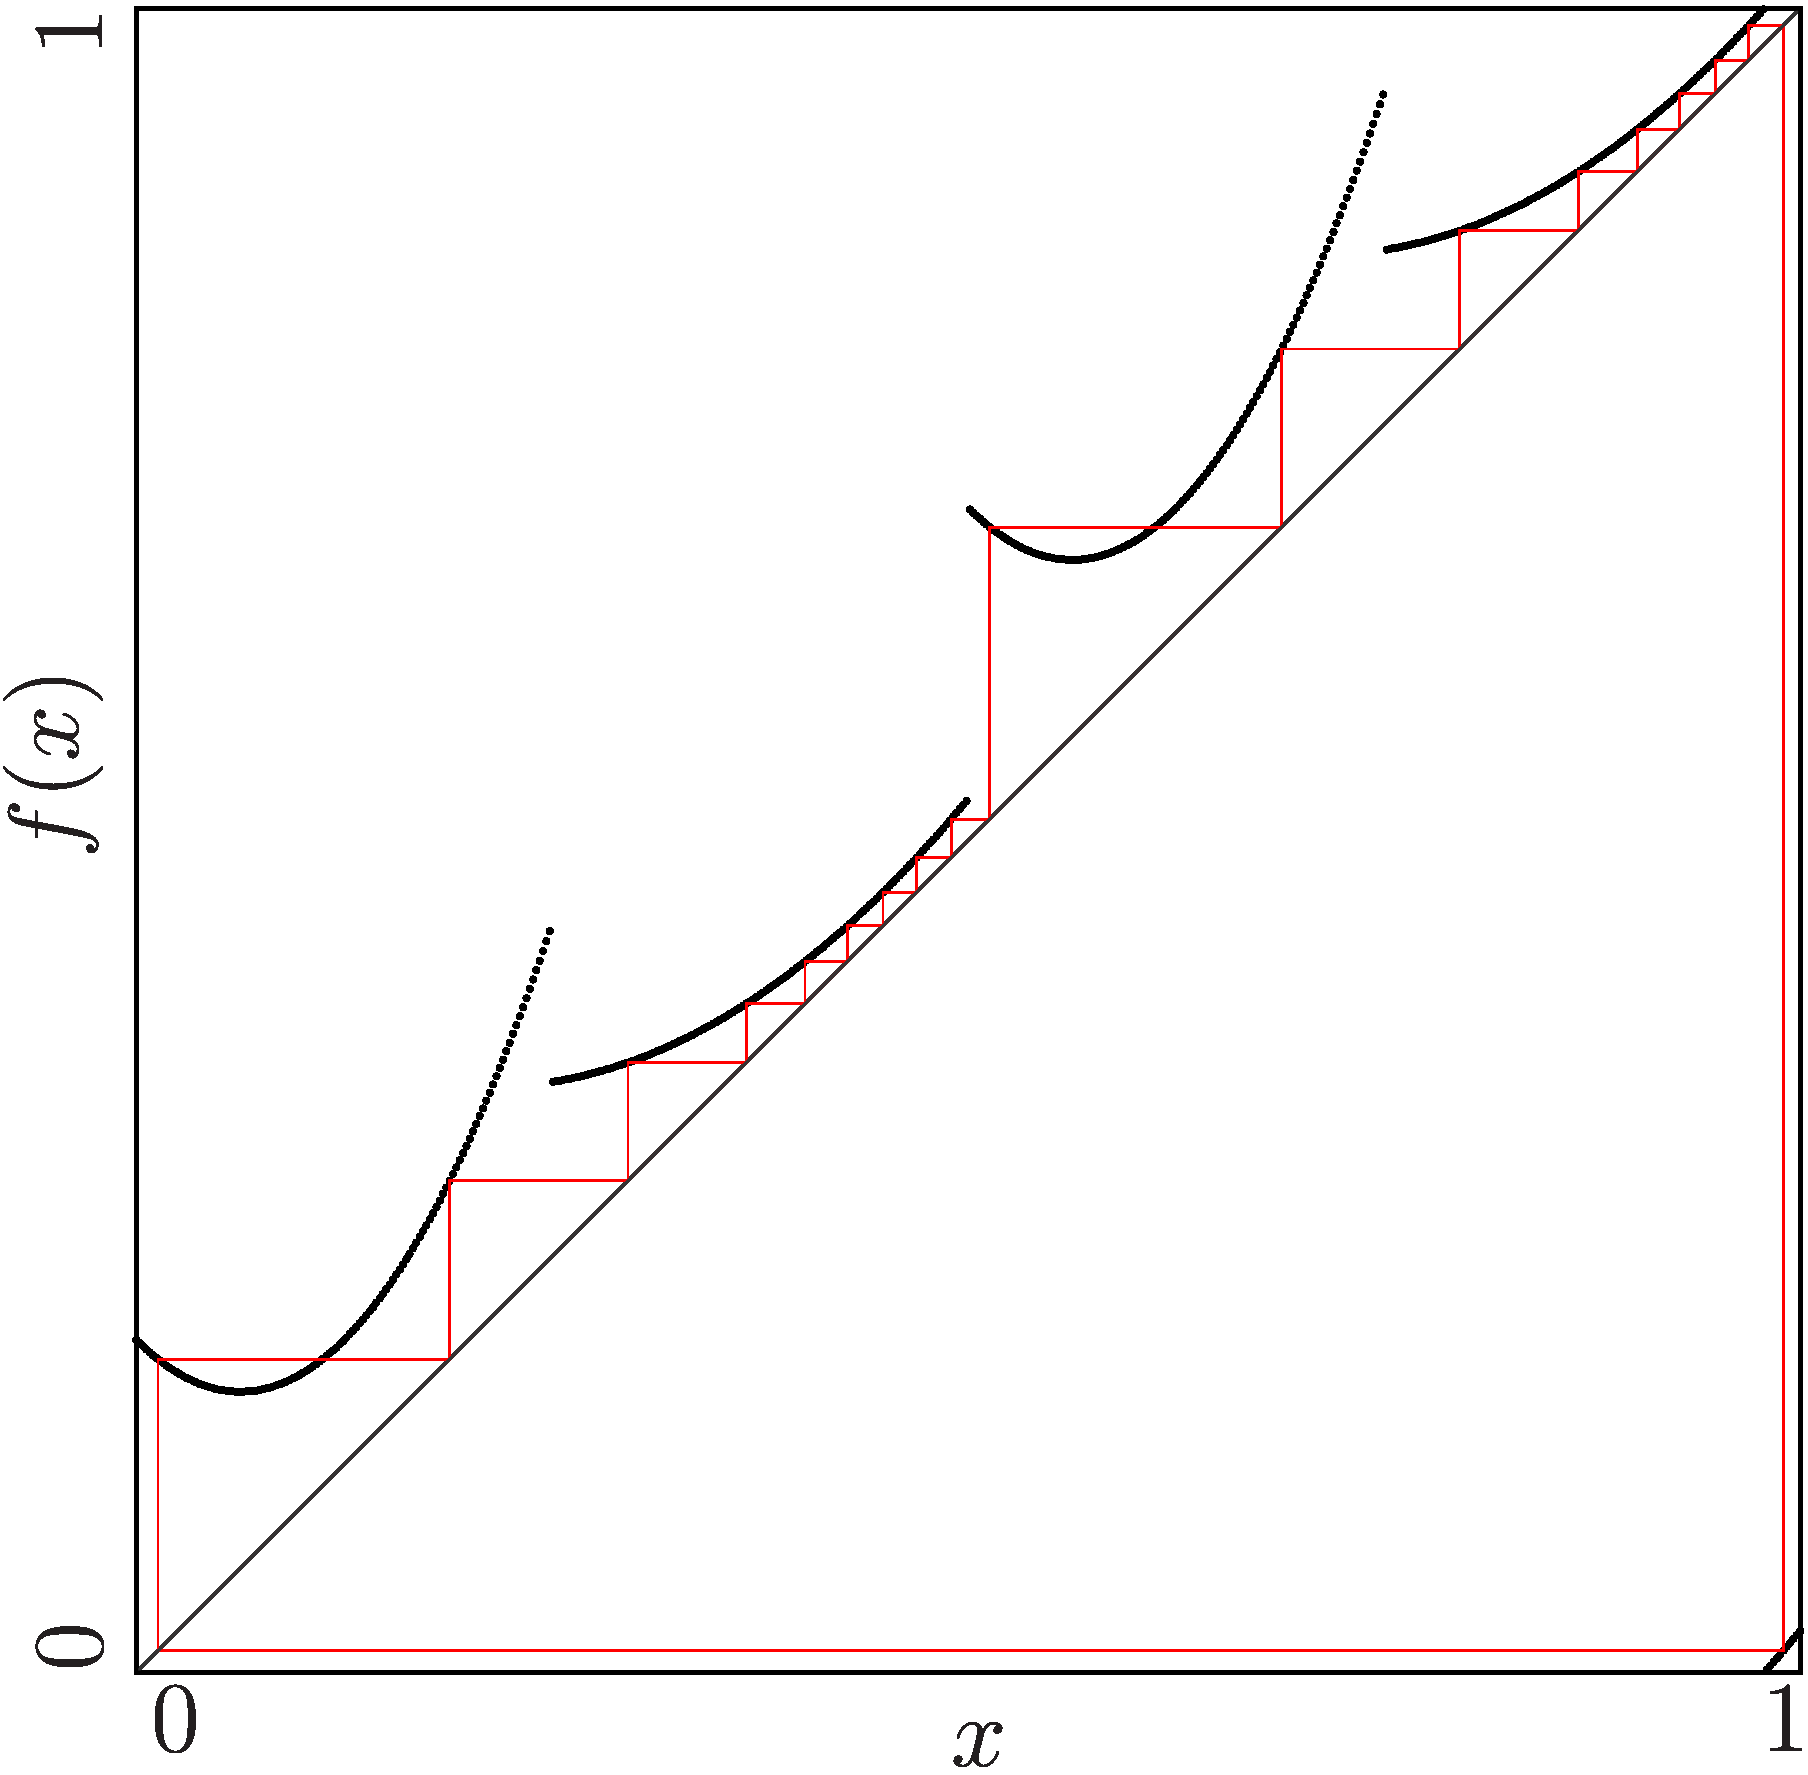
\includegraphics[width=.3 \textwidth]{../Figures/5/5.10c/result.png}
		\label{fig:setup.quad.hyper.1.cobweb.C}
	}
	\caption[Cobweb diagrams of the first piecewise quadratic model with composite parameters]{
	Cobweb diagrams at three parameter values of $\alpha = g_R\left(\frac{1}{4}\right)$ and $\beta = c_L$ in the piecewise quadratic model with hyperparameters.
	The other parameters are fixed as $a_L = 8, b_L = -1, g_R\left(\frac{1}{2}\right) = \frac{1}{2} + \frac{1}{40}$, and $\left. \frac{d}{dx} g_R(x) \right|_{x = \frac{1}{2}} = 1 + \frac{1}{5}$.
	The parameter values are marked in \Cref{fig:setup.quad.hyper.1.period}.
	(a) shows the cycle $\Cycle{\A^4\B^5\C^4\D^5}$ at the point $A$ where $\alpha = 0.42$ and $\beta = 0.1525$,
	(b) shows the cycle $\Cycle{\A^3\B^6\D^3\C^6}$ at the point $B$ where $\alpha = 0.385$ and $\beta = 0.1675$,
	and (c) shows the cycle $\Cycle{\A^2\B^7\C^2\D^7}$ at the point $C$ where $\alpha = 0.385$ and $\beta = 0.1675$.
	}
	\label{fig:setup.quad.hyper.1.cobwebs}
\end{figure}

\Cref{fig:setup.quad.hyper.1.period} shows a 2D scan of the periods associated with parameter regions in the specified parameter range for $\alpha$ and $\beta$.
At the top, some periods are annotated.
One can see that in the scan there are sequences of parameter regions that are associated with the same period.
These sequences are next to each other, where each sequence is associated with a period that is two numbers higher than the period associated with the parameter region sequence right of it.
This is similar to the \gls{pi} that can be observed in the original model, as described in \Cref{sec:state.og.dynamics}.
One difference is that the sequences in the original model were connected and formed chains.

\Cref{fig:setup.quad.hyper.1.cobwebs} shows cobweb diagrams for different parameter values along the sequence of parameter regions associated with the period $18$.
These parameter values are marked with points in \Cref{fig:setup.quad.hyper.1.period}.
\Cref{fig:setup.quad.hyper.1.cobweb.A} shows the cycle at the point $A$ with the symbolic sequence $\A^4\B^5\C^4\D^5$.
\Cref{fig:setup.quad.hyper.1.cobweb.B} shows the cycle at the point $B$ with the symbolic sequence $\A^3\B^6\C^3\D^6$.
Notice that the cycle at point $B$ has one point less on the branches $f_\A$ and $f_\C$ each than the cycle at point $A$, while it has one point more on the branches $f_\B$ and $f_\D$ each.
It is as if two points, one of each of the branches $f_\A$ and $f_\C$, moved to the next branch from one parameter region of the sequence to the next.
\Cref{fig:setup.quad.hyper.1.cobweb.C} shows the cycle at the point $B$ with the symbolic sequence $\A^2\B^7\C^3\D^7$.
Again, two points, one of each of the branches $f_\A$ and $f_\C$, moved to the next branch from the parameter region with point $B$ to the parameter region with the point $C$.
This is also very similar to the behavior of the original model, where two points, one of each of the branches $F_\A$ and $F_\C$, moved to the next branch each along the chain of parameter regions associated with the same period, as described in \Cref{sec:state.og.dynamics}.
Besides that the sequences of parameter region associated with the same period are not connected here, there is another difference to the behavior of the original model.
In the original model there are ``type B'' parameter regions between the ``type A'' parameter regions of a chain of parameter regions with the same period.
To reiterate, ``type A'' parameter regions are associated with a single symmetric cycle.
These are the parameter regions, one can observe in this case also.
Between two ``type A'' parameter regions there is a parameter region that is associated with two coexisting asymmetrical twin cycles, called ``type B'' parameter regions.
These ``type B'' parameter regions are missing in this case.

\subsection{Shallow Parabola-shaped Branches $f_\A$ and $f_\C$}
\label{sec:setup.quad.hyper.2}

To close the gaps in between the parameter regions in the sequences, the parameters of the function $g_L$ that governs the shape of the branches $f_\A$ and $f_\C$ is adjusted.
The new fixed parameter values are $a_L = 4$ and $b_L = -\frac{1}{2}$.
And the other fixed parameters stay the same as in the previous section.

One can see in \Cref{fig:setup.quad.hyper.1.cobwebs} that the shape of the branches $f_\A$ and $f_\C$ is very steep.
This is different from the branches $F_\A$ and $F_\C$ in the original model that were more shallow.
The new fixed parameter values of $a_L$ and $b_L$ also cause the shape of the branches $f_\A$ and $f_\C$ to be more shallow.
One can see this in the cobweb diagrams in \Cref{fig:setup.quad.hyper.2.cobwebs}.
The varied parameters are the same as in the previous section and therefore the parameter effects of $E_0$ and $\chi_0$ on the original model function are emulated well.
This was thoroughly described in the previous section, \Cref{sec:setup.quad.hyper.1}.

\Cref{fig:setup.quad.hyper.2.period} shows 2D scans of periods associated with parameter regions in this model.
It shows 2 different versions of scans in the same parameter range, $\alpha \in [0.275, 0.35]$ and $\beta \in [0.15, 0.1875]$.
The first scan in \Cref{fig:setup.quad.hyper.2.period.full} shows the periods of the model as we have seen it also in the previous sections.
The second scan in \Cref{fig:setup.quad.hyper.2.period.halved} shows the periods of the same model but halved.
This reveals ``type B'' parameter regions as they are associated with higher periods than the ``type A'' parameter regions of the same chains in the halved model.
The reason for this is covered in-depth in \Cref{sec:add.add.halved}, but for now only the fact that it reveals ``type B'' parameter regions is important.

We can see in \Cref{fig:setup.quad.hyper.2.period.full}, that the gap between the ``type A'' parameter regions of a sequence of parameter regions associated with the same period closed.
Also, there are sections of the chains where they get narrower, for example at point $C$.
In the original model one can observe the same narrowing of the chains.
These narrower sections are ``type B'' parameter regions in the original model.


\Cref{fig:setup.quad.hyper.2.period.halved} reveals ``type B'' parameter regions in the quadratic model with compound parameters.
We can see that ``type A'' and ``type B'' parameter regions alternate in the chains of parameter regions associated with the same period.
Also, the ``type B'' parameter regions are at the narrower sections of the chains.
This is exactly the same behavior one can observe in the original model when examining the types of the parameter regions making up the chains and their arrangement.

The period the chains are associated with also still increments in neighboring chains as was observed in the last section, \Cref{sec:setup.quad.hyper.1}.
Therefore, this structure is similar to the \gls{pi} structure one can observe in the original model when looking at the periods associated with parameter regions and their types.
But this is not the only characteristic of cycles.
Therefore, the symbolic sequences of the cycles associated with the parameter regions making up the chains are analyzed next.

\begin{figure}
	\centering
	\subfloat[Model]{
		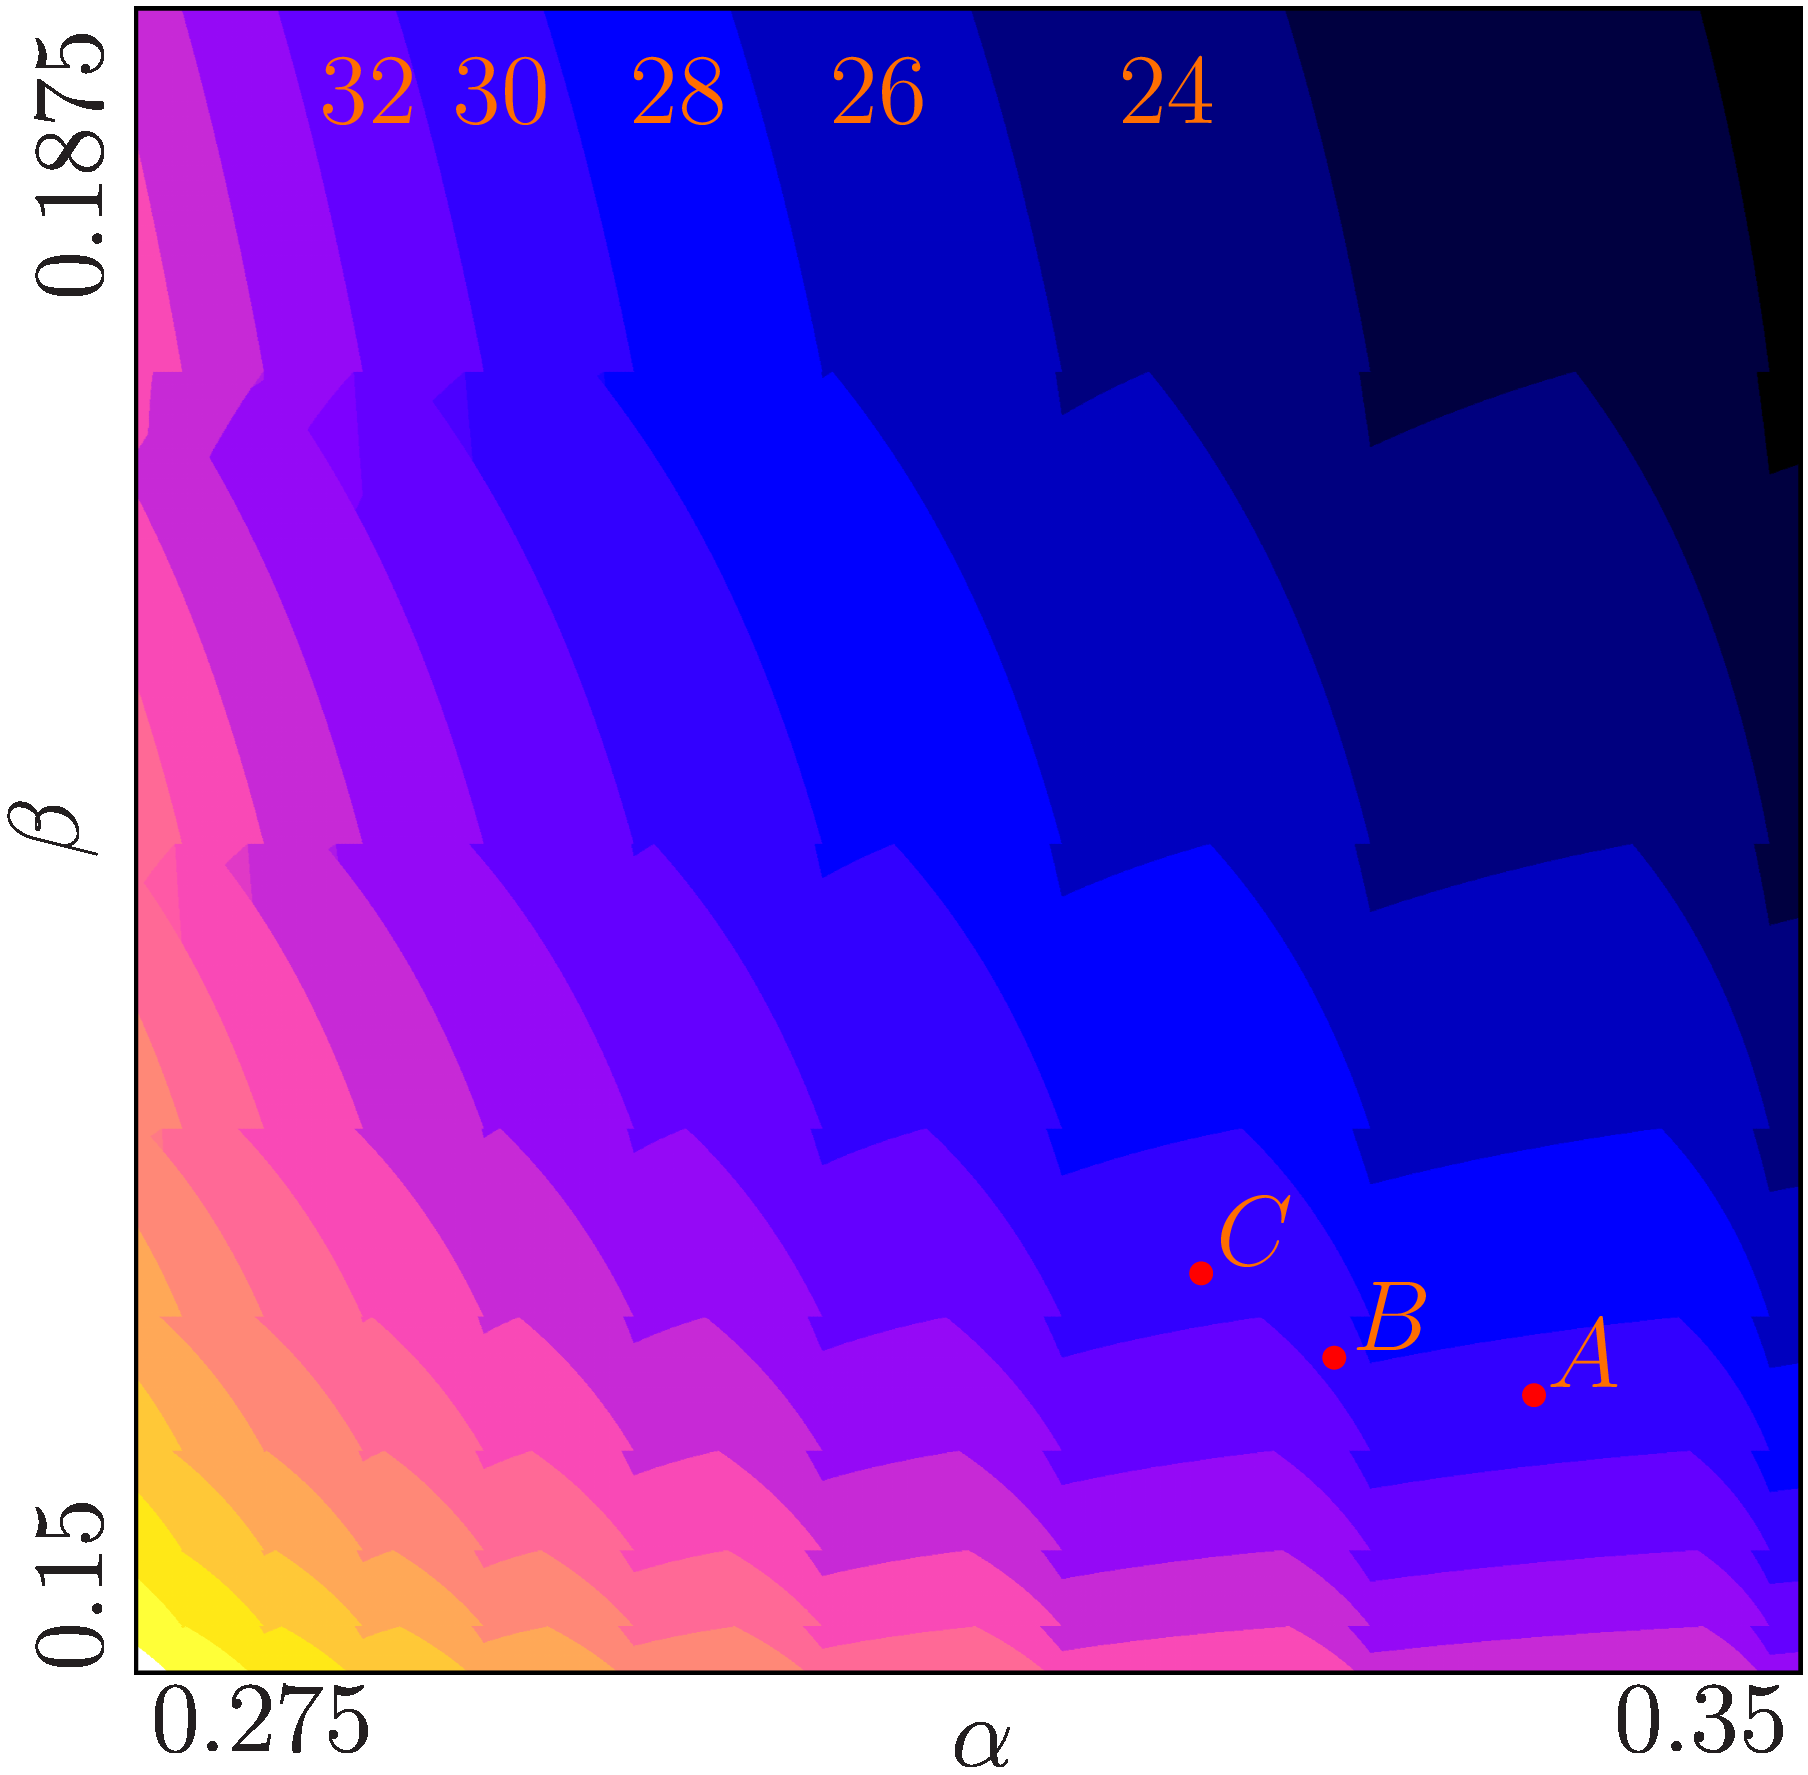
\includegraphics[width=.48 \textwidth]{../Figures/5/5.11a/result.png}
		\label{fig:setup.quad.hyper.2.period.full}
	}
	\subfloat[Halved model]{
		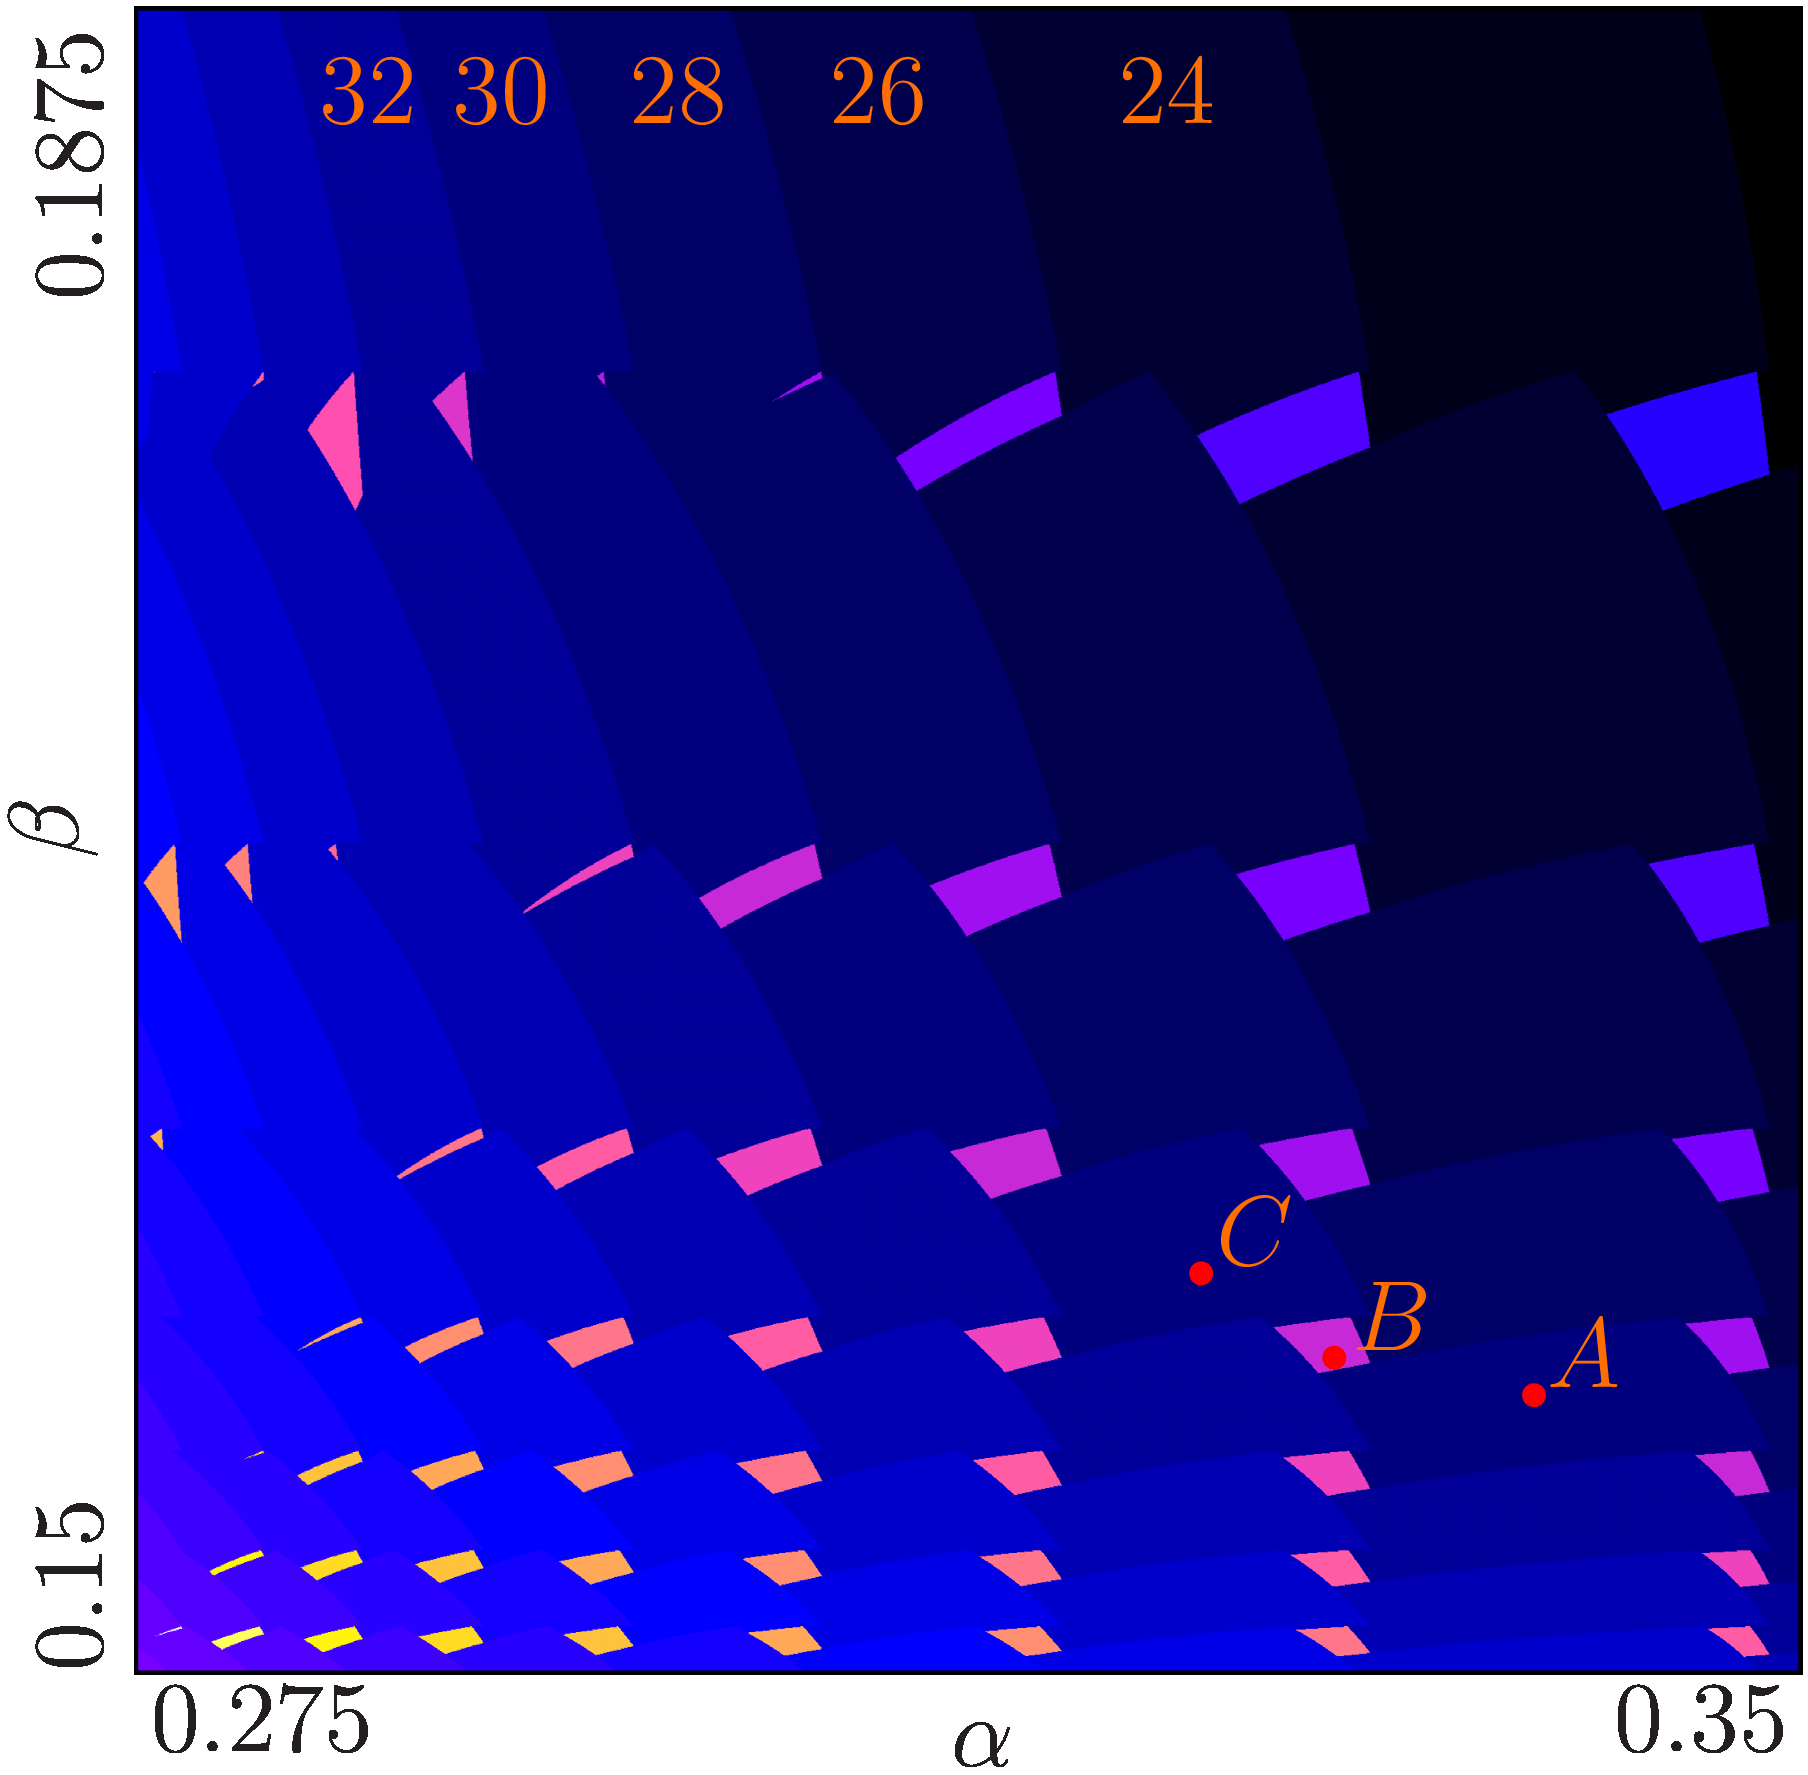
\includegraphics[width=.48\textwidth]{../Figures/5/5.11b/result.png}
		\label{fig:setup.quad.hyper.2.period.halved}
	}
	\caption[2D scan of the periods of the quadratic model with hyperparameters for different values of the fixed parameters]{
	2D scan of the periods of the piecewise quadratic model with hyperparameters $g_R\left(\frac{1}{4}\right), g_R\left(\frac{1}{2}\right),$ and $\left. \frac{d}{dx} g_R\left(x\right) \right|_{x = \frac{1}{2}}$.
	The parameters $a_L = 4, b_L = -\frac{1}{2}, g_R\left(\frac{1}{2}\right) = \frac{1}{2} + \frac{1}{40},$ and $\left. \frac{d}{dx} g_R\left(x\right) \right|_{x = \frac{1}{2}} = 1.2$ are fixed.
	The parameters $\alpha = g_R\left(\frac{1}{4}\right)$ and $\beta = c_L$ are varied in the ranges $[0.275, 0.35]$ and $[0.15, 0.1875]$, respectively.
	The points $A, B,$ and $C$ mark the parameter values used for the cobweb diagrams in \Cref{fig:setup.quad.hyper.2.cobwebs}.
	Also, the numbers at the top indicate the period of the parameter region chains.
	(a) shows the scan for the model as defined above, while (b) shows the scan for the halved model where we can see ``type B'' parameter regions as they have higher periods than the ``type A'' parameter regions of the same chain.
	}
	\label{fig:setup.quad.hyper.2.period}
\end{figure}

\begin{figure}
	\centering
	\subfloat[$A$]{
		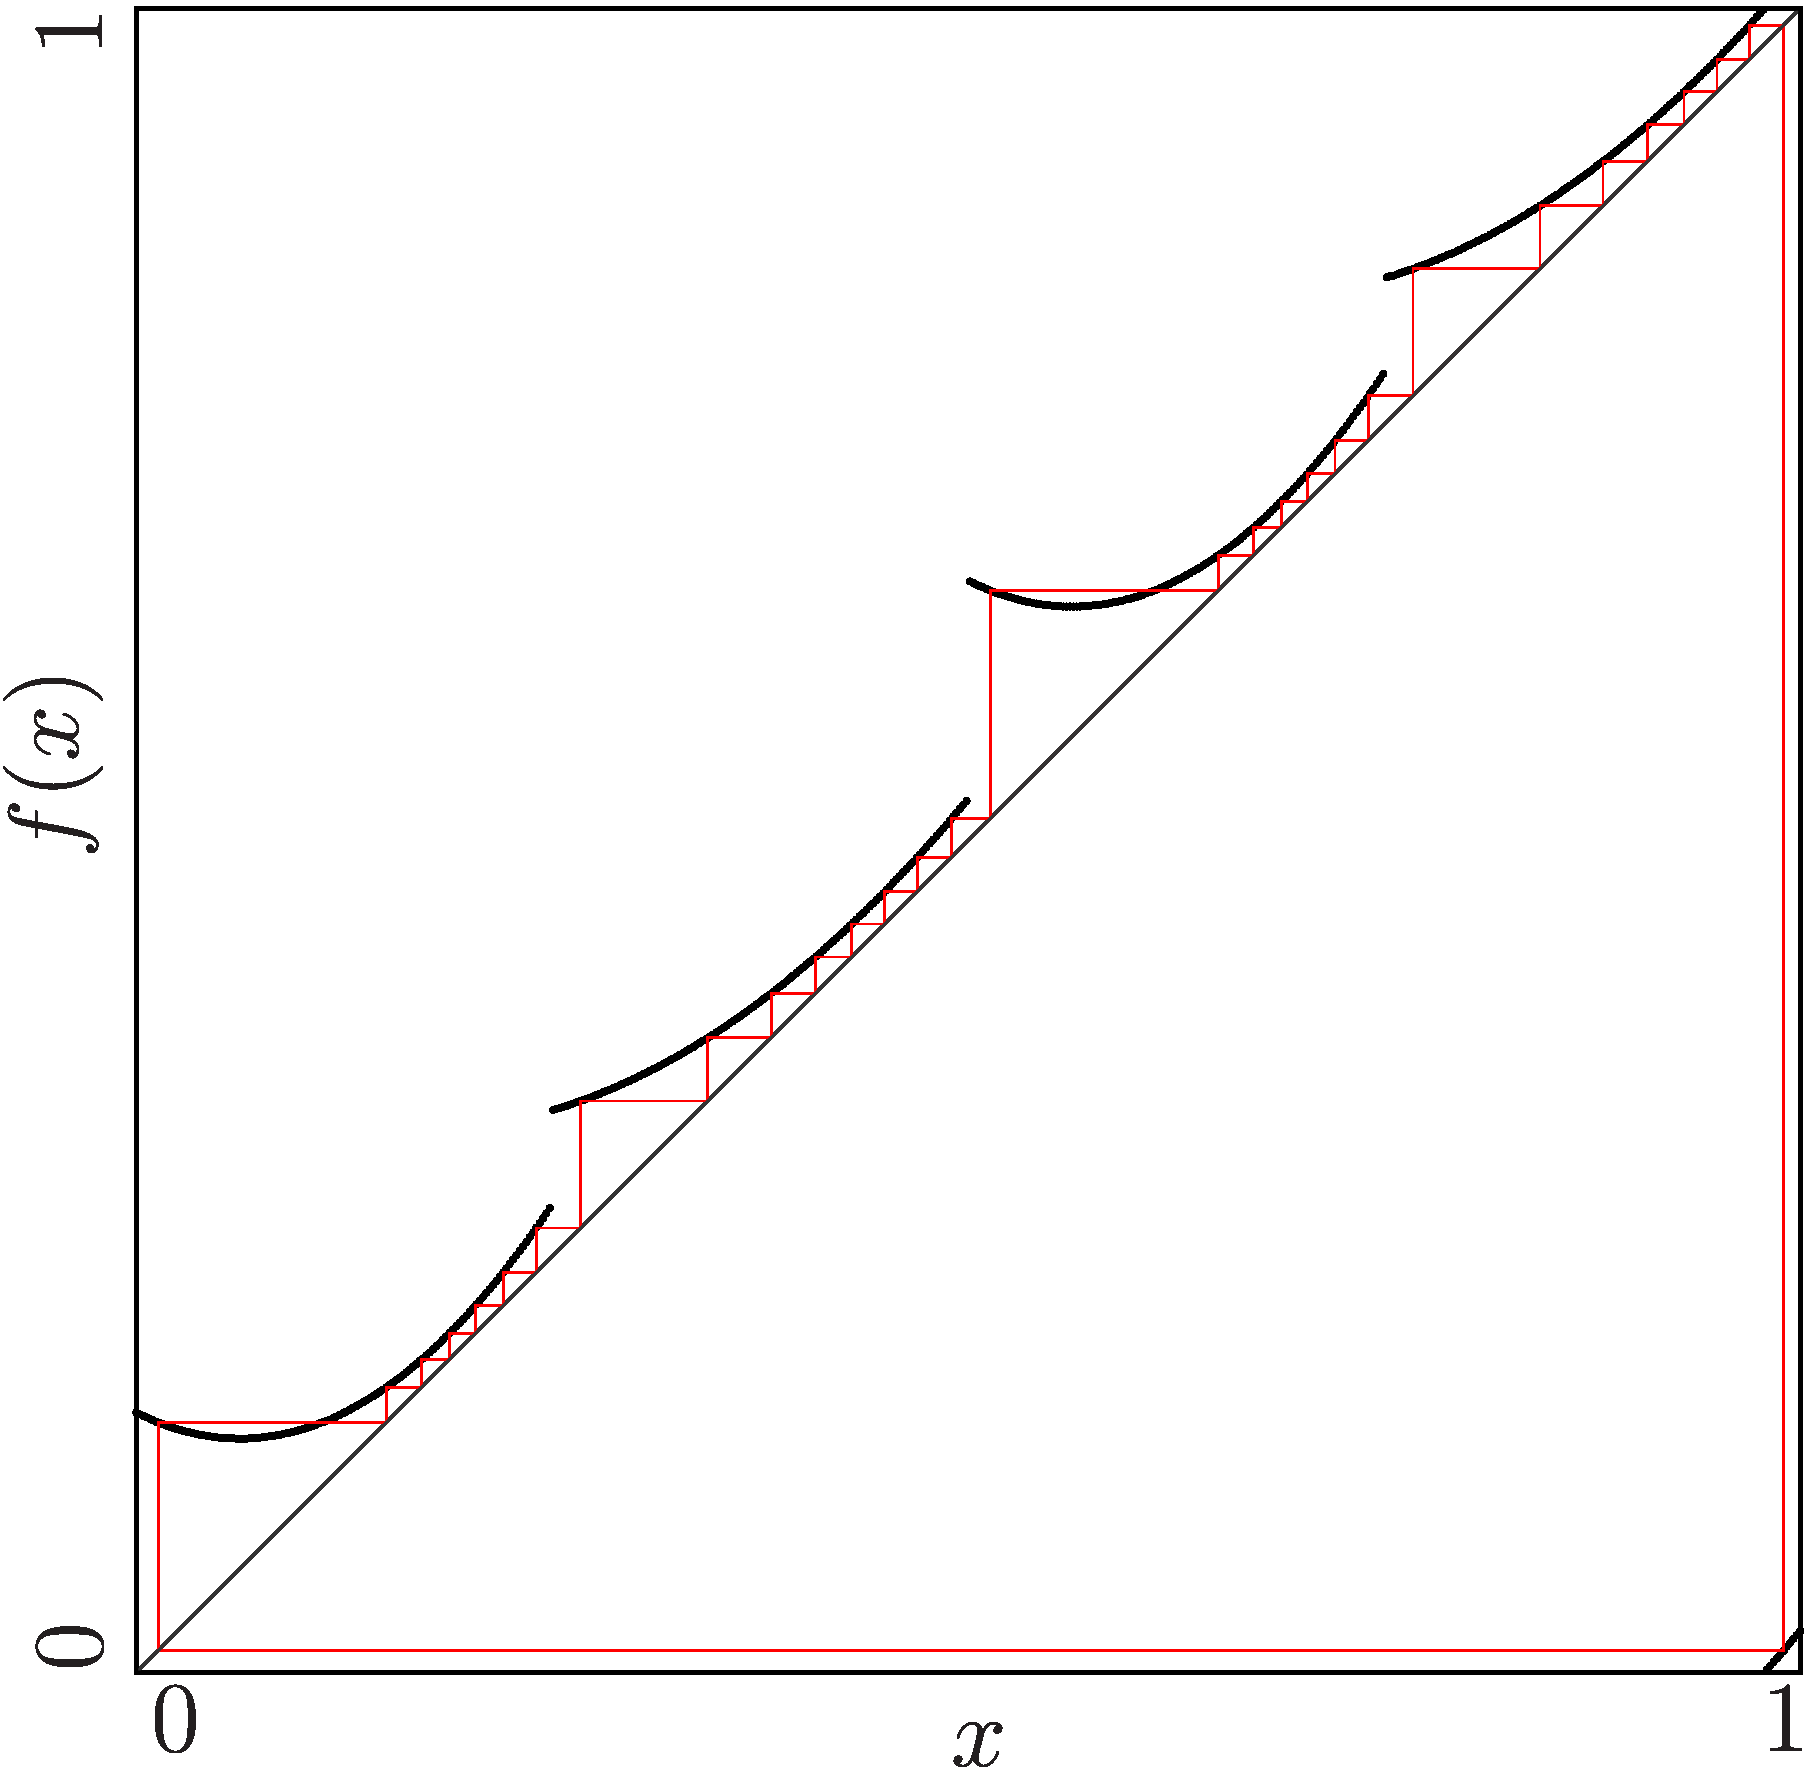
\includegraphics[width=.3 \textwidth]{../Figures/5/5.12a/result.png}
		\label{fig:setup.quad.hyper.2.cobweb.A}
	}
	\subfloat[$B$]{
		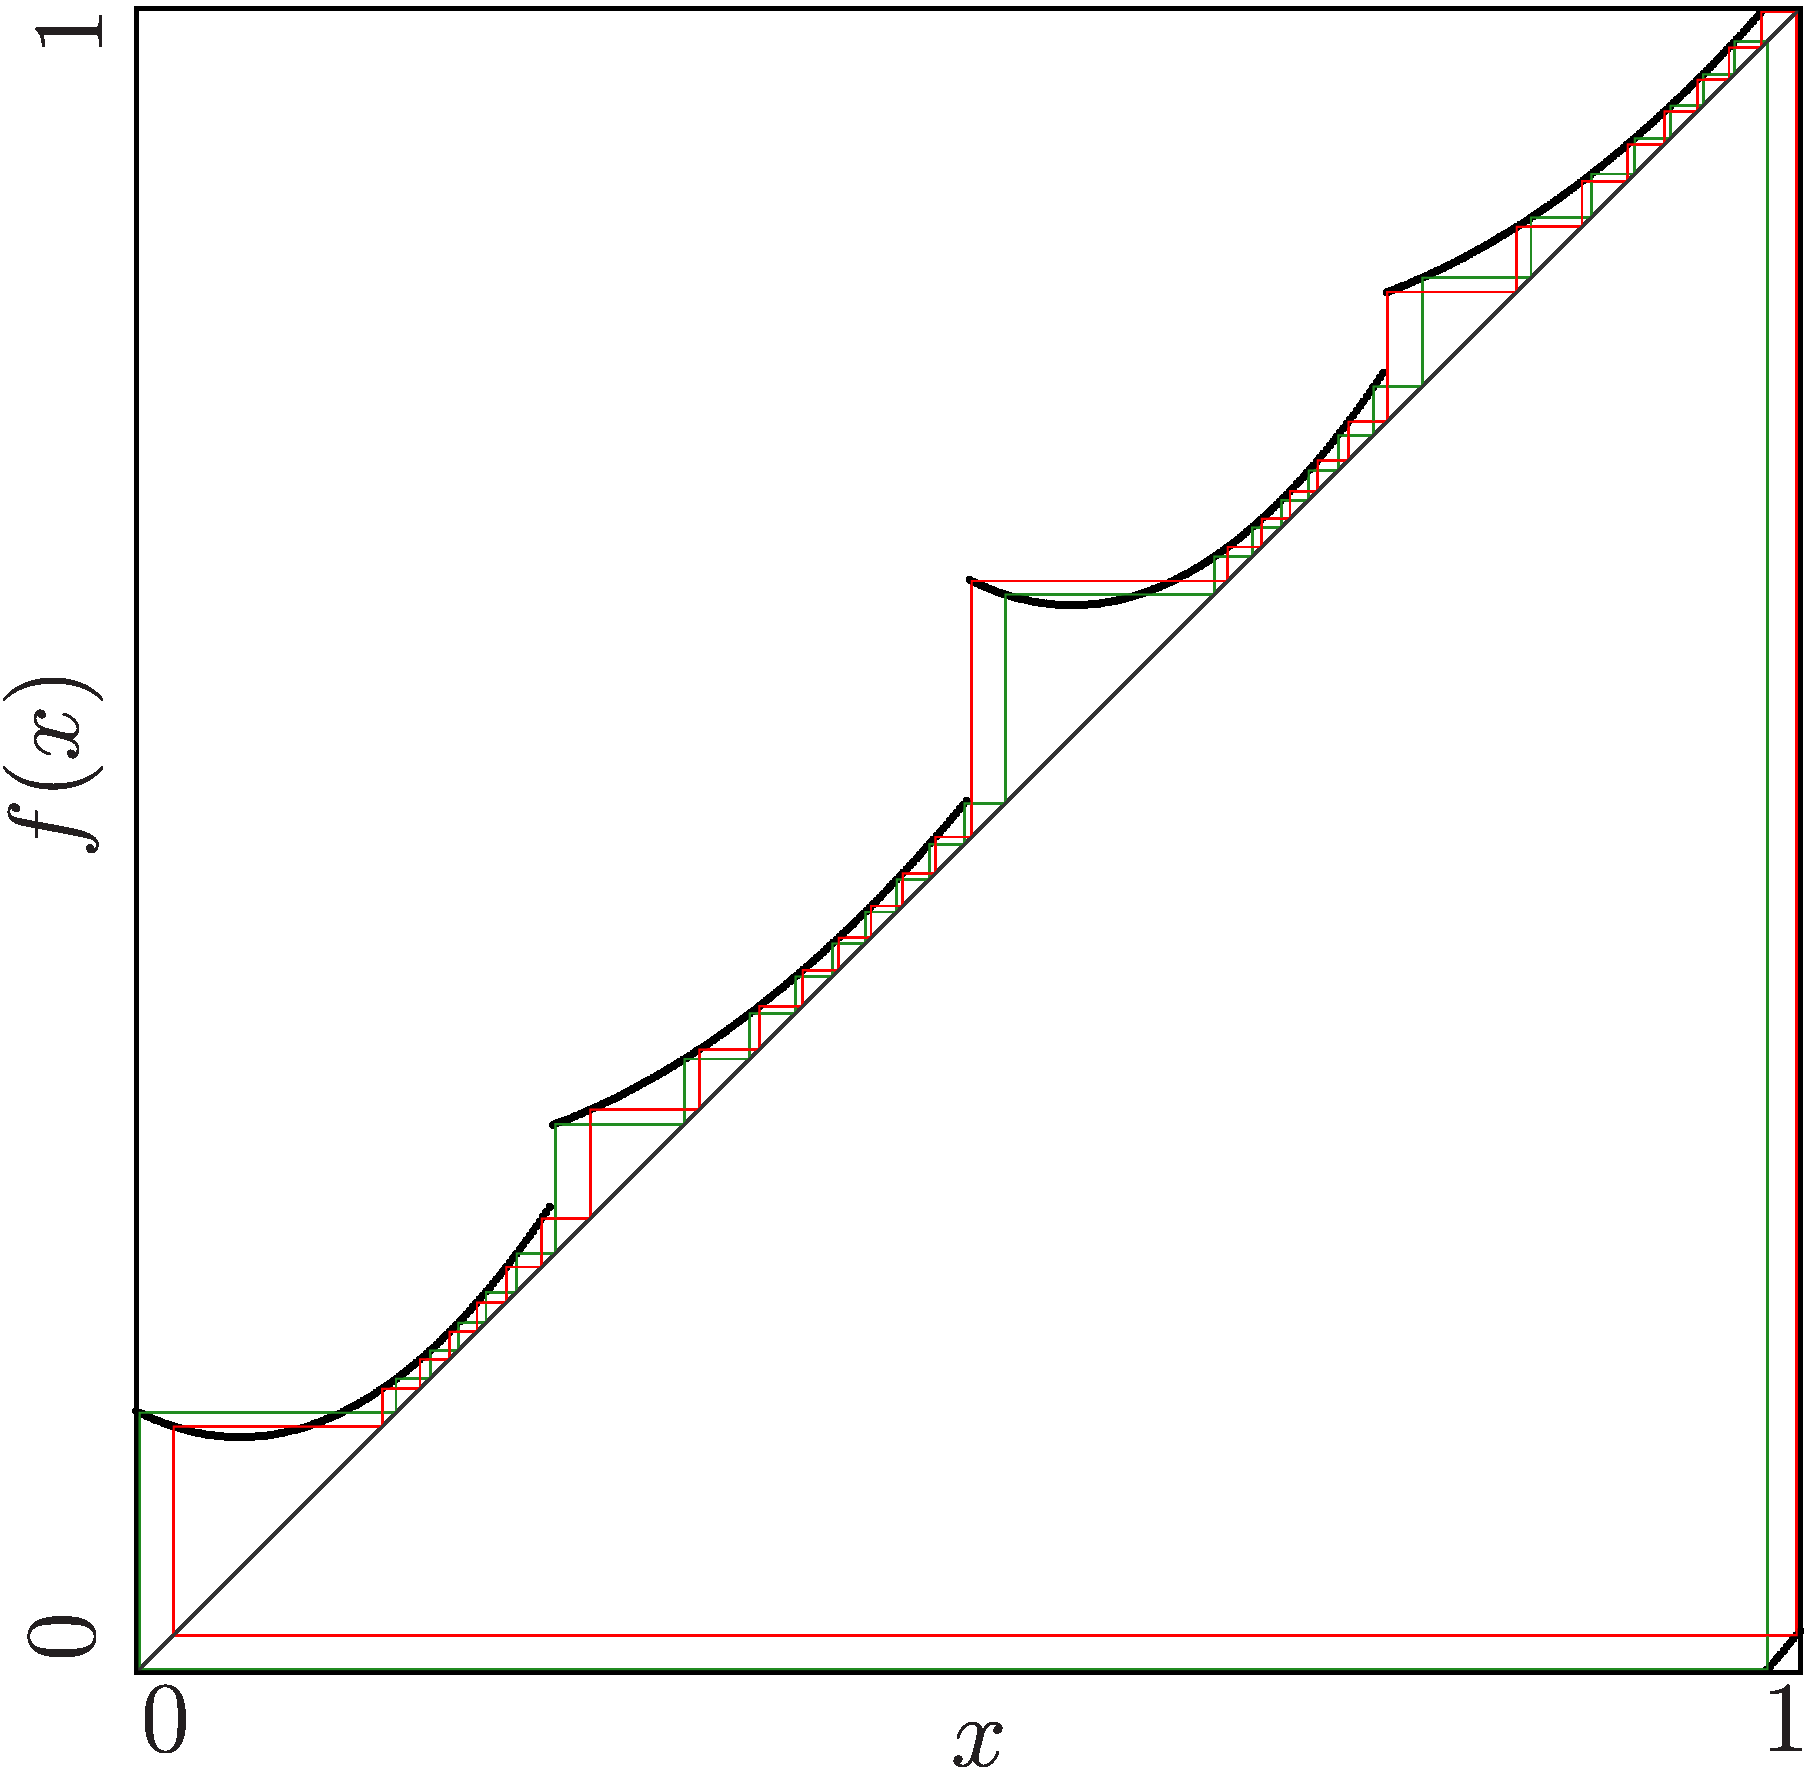
\includegraphics[width=.3 \textwidth]{../Figures/5/5.12b/result.png}
		\label{fig:setup.quad.hyper.2.cobweb.B}
	}
	\subfloat[$C$]{
		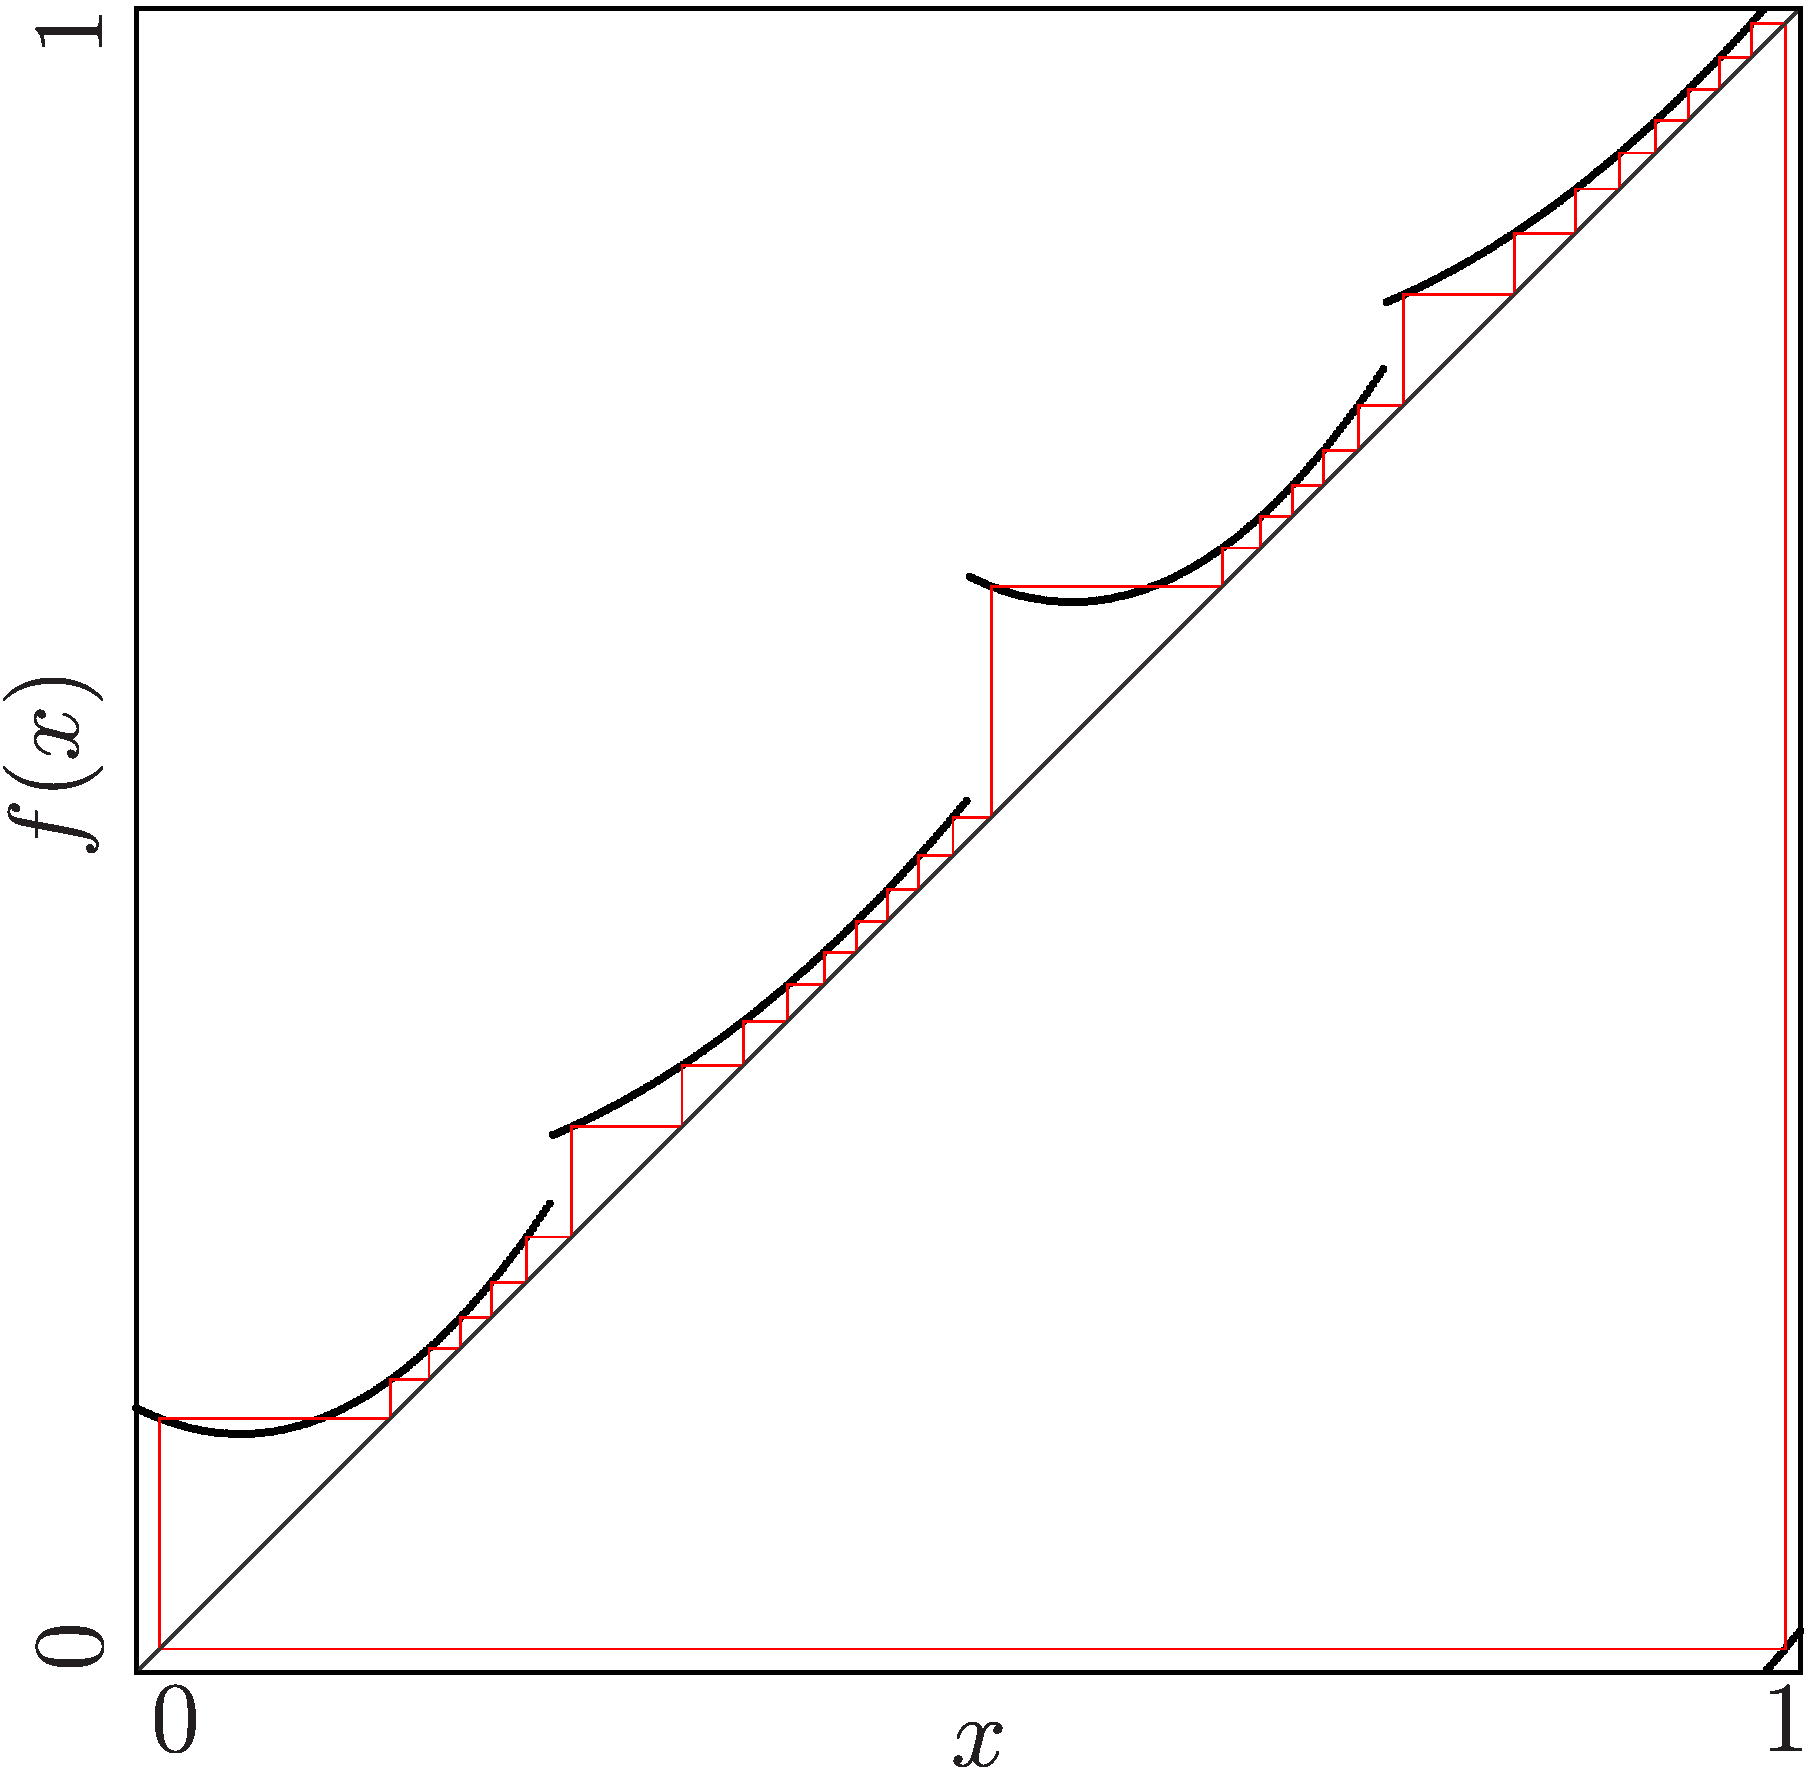
\includegraphics[width=.3 \textwidth]{../Figures/5/5.12c/result.png}
		\label{fig:setup.quad.hyper.2.cobweb.C}
	}
	\caption[Cobwebs of the piecewise quadratic model with hyperparameters for different values of the fixed parameters]{
	Cobweb diagrams at three parameter values of $\alpha = g_R\left(\frac{1}{4}\right)$ and $\beta = c_L$ in the piecewise quadratic model with hyperparameters.
	The other parameters are fixed as $a_L = 4, b_L = -\frac{1}{2}, g_R\left(\frac{1}{2}\right) = \frac{1}{2} + \frac{1}{40}$, and $\left. \frac{d}{dx} g_R(x) \right|_{x = \frac{1}{2}} = 1 + \frac{1}{5}$.
	The parameter values are marked in \Cref{fig:setup.quad.hyper.2.period}.
	(a) shows the cycle $\Cycle{\A^7\B^8\C^7\D^8}$ the at point $A$where $\alpha = 0.338$ and $\beta = 0.15625$,
	(b) shows the two coexisting cycles $\Cycle{\A^7\B^8\C^7\D^8}$ (green) and $\Cycle{\A^6\B^9\C^6\D^9}$ (red) at the point $B$where $\alpha = 0.329$ and $\beta = 0.1571$,
	and (c) shows the cycle $\Cycle{\A^6\B^9\C^6\D^9}$ at the point $C$where $\alpha = 0.323$ and $\beta = 0.159$.
	}
	\label{fig:setup.quad.hyper.2.cobwebs}
\end{figure}

\Cref{fig:setup.quad.hyper.2.cobwebs} contains the cobweb diagrams for the cycles at the parameter values that are marked with points $A, B,$ and $C$ in \Cref{fig:setup.quad.hyper.2.period}.
This chain of parameter regions is associated with the period $30$, therefore all the cycles shown here also have the period $30$.
The symbolic sequence of the cycle at point $A$ is $\A^7\B^8\C^7\D^8$.
It is a symmetric cycle and therefore the parameter region is of ``type A''.
The symbolic sequence of the cycle at point $C$ is $\A^6\B^9\C^6\D^9$.
It is also a symmetric cycle and this parameter region is also of ``type A''.
The parameter region with point $C$ is the next ``type A'' parameter region after the parameter region with point $A$ in the chain.
And just like in the original model, one point of each of the branches $f_\A$ and $f_\C$ moved to the next branch.

Between those two ``type A'' parameter regions there is a narrower ``type B'' parameter region with the same period.
It is marked with the point $C$.
At this point, there are 2 coexisting cycles with the period 30.
Their symbolic sequences are $\A^7\B^8\C^6\D^9$ and $\A^6\B^9\C^7\D^8$, respectively.
This is exactly the same behavior that one can observe in the original model.
Between two ``type A'' parameter regions with the cycles $\Cycle{\A^a\B^b\C^c\D^d}$ and $\Cycle{\A^c\B^d\C^c\D^d}$ there is a ``type B'' parameter region with the two coexisting cycles $\Cycle{\A^a\B^b\C^c\D^d}$ and $\Cycle{\A^c\B^d\C^c\D^d}$.
Where $c = a - 1$ and $d = b + 1$.

Therefore, the bifurcation structure in this model fulfills all criteria, although it is mirrored.
In the \gls{pi} structure in the original model, the periods increased from left to right, here they increase from right to left.
Also, the chains start in the lower left corner and go towards to the upper right corner, here they start in the lower right corner and go towards the upper left corner.
But the model can still be simplified.
The branches $f_\B$ and $f_\D$ are only increasing and almost linear.
One can observe this in the cobweb diagrams in \Cref{fig:setup.quad.hyper.2.cobwebs}.

